\chapter{Posit numbers}\label{chap:posit_num}
\lettrine{P}{osit} numbers made their first appearance in the work of John L. Gustfason "Beating Floating Point at its Own Game: Posit Arithmetic" \cite{gustafson2017beating}. The idea behind the format was to create a drop-in replacement for binary32 numbers. Posit numbers can be also seen as a new iteration of Universal Numbers (also called \textit{unum}). We can consider Posits as Type III unums.
Type I unums are a super-set of binary32 numbers, that is extended with an additional bit, called \textit{ubit}, that states whether the real number represented by that Unum is an exact binary32 or lies between two consecutive representations. Another difference with binary32 numbers is that unums do not have a predefined length for exponent and fraction fields. 

The second iteration of Type I unums - namely, Type II unums - points in the direction of totally abandoning the compatibility with binary32 numbers, nearing the concept of \textit{projective reals}\footnote{\url{https://en.wikipedia.org/wiki/Real_projective_line}}. The final iteration of unums is represented by the Type III Unum, also called Posit.


\section{Format and general properties}

Posit numbers are stored in two's complement integers. As shown in Figure \ref{fig:positFormat}, a Posit number is comprised of at most four fields. It can be configured on two parameters: the number of total bits \textit{nbits} and the maximum number of exponent bits \textit{esbits}
\begin{itemize}
    \item  \textcolor{asparago}{S} is the sign bit as commonly used in IEEE binary formats.
    \item \textcolor{amber}{Regime} is the regime field, on variable length; it can take up to the entire bit-space of the format after the sign bit.
    \item \textcolor{lightred}{Exponent} is the exponent field, without any bias offset; depending on $esbits$ and regime length it can span from $0$ to $esbits$ bits.
    \item \textcolor{lightgreen}{Fraction} is the fractional part of the mantissa; depending on the other fields it can be absent.
\end{itemize}
Sign, exponent and fraction have the same identical meaning as the homonymous fields in IEEE binary numbers. 
The regime field is instead new and different: its length depends on the value of the bits. In particular, the regime length depends on the number of subsequent identical bits that we find after the sign until a bit of opposite value is found. This means that, if we have this bit-string:
\begin{equation}
    b_1, b_2, b_3 \dots b_l, \overline{b_{l}}
\end{equation}
 where $b_1 = b_2 = \dots = b_l = b$, the regime length will be $l$. Depending on the value of $b$ the regime value $k$ will be computed as follows:
\begin{equation}\label{eqn:regimeValue}
k = \left\{\begin{matrix}
 l-1& b = 1  \\
 -l & b = 0  \\
\end{matrix}\right.
\end{equation}
The regime value is a scale factor for a special constant, that depends on the posit configuration, called \textit{useed}. The \textit{useed} value is computed as follows:
\begin{equation}\label{eqn:useed}
    \text{useed} = 2^{2^{esbits}}
\end{equation}

Wrapping everything up, the real value associated with a posit $p$ represented by the integer $P$ on two's complement (with sign $s$) is computed as in Equation \eqref{eqn:positRealValue}. The value $F$ is the length of the fraction field. Note that there will be always an implicit $1.$ in front of the fraction (i.e. $1.f_1,f_2, \dots, f_F$), without any subnormal number differently from IEEE binary numbers.

\begin{equation}\label{eqn:positRealValue}
 r =   \left\{\begin{matrix}
0 & P = 0  \\
\pm \infty & P = -2^{nbits-1}  \\
(-1)^s \cdot \text{useed}^{k} \cdot 2^e \cdot \left ( 1+ \frac{f}{2^F} \right) &  \text{otherwise} \\
\end{matrix}\right.
\end{equation}


Having the exponent and the fraction bits depending on the length of the regime is a clever way to express the so-called \textit{tapered accuracy}: numbers near $1$ (in magnitude) will have more bits allocated for the fractional part than extremely large (or small) numbers farther from $1$, thus having higher decimal accuracy. Although it highly depends on the application, the probability of encountering such extremely large or small numbers is far smaller than the one for numbers near to 1. This theoretically gives a substantial boost to posit accuracy in computations.
Figures \ref{fig:positCloseToOne} and \ref{fig:positFarFromOne} show this concept with an example. The real value $1.125$ is closer to $1$ than the value $32704$: as we can see, the number of fraction bits in the former is far greater than the one on the latter. This also reflects on the \textit{denominator} of the fraction, being $2048$ in the case of the real value $1.125$ and a quarter of that i.e. $256$ for the real value $32704$.

\begin{figure}[t]
	\centering    
    \begin{bytefield}[bitwidth=1em]{32}
       \colorbitbox{asparago}{1}{{\scriptsize{S}}}&
       \colorbitbox{amber}{10}{\scriptsize{Regime(1..$rebits$)}} &
       \colorbitbox{lightred}{9}{\scriptsize{Exponent (0..$esbits$)}} &
       \colorbitbox{lightgreen}{12}{\scriptsize{Fraction (0...)}} 
    \end{bytefield}
    \caption{The posit format}
	\label{fig:positFormat}
\end{figure}


\begin{figure}\centering\begin{bytefield}[bitwidth=0.66em]{16}\bitbox{16}{0\,1\,0\,0\,0\,0\,0\,1\,0\,0\,0\,0\,0\,0\,0\,0}\\\\\bitheader[endianness=big]{0-15}\\\colorbitbox{lightcyan}{1}{{S}}&\colorbitbox{lightgreen}{2}{R}&\colorbitbox{lightred}{2}{E}\colorbitbox{amber}{11}{F}\\\bitbox{1}{\color{cyan}0}&\bitbox{2}{\color{amber}1\!\;\color{darkamber}0}&\bitbox{2}{\color{lightred}0\!\;0}&\bitbox{11}{\color{darkgreen}0\!\;0\!\;1\!\;0\!\;0\!\;0\!\;0\!\;0\!\;0\!\;0\!\;0}&\end{bytefield}\caption{An example of Posit configuration with 16 bits and 2 exponent bits. The associated real value to the shown Posit is:$\textcolor{cyan}{1}\cdot 16^{\textcolor{darkamber}{0}}\cdot 2^{\textcolor{lightred}{0}}\cdot ( 1 + \textcolor{darkgreen}{256}/2048)= 1.125$}\label{fig:positCloseToOne}\end{figure}

\begin{figure}\centering\begin{bytefield}[bitwidth=0.66em]{16}\bitbox{16}{0\,1\,1\,1\,1\,0\,1\,0\,1\,1\,1\,1\,1\,1\,1\,1}\\\\\bitheader[endianness=big]{0-15}\\\colorbitbox{lightcyan}{1}{{S}}&\colorbitbox{lightgreen}{5}{R}&\colorbitbox{lightred}{2}{E}\colorbitbox{amber}{8}{F}\\\bitbox{1}{\color{cyan}0}&\bitbox{5}{\color{amber}1\!\;1\!\;1\!\;1\!\;\color{darkamber}0}&\bitbox{2}{\color{lightred}1\!\;0}&\bitbox{8}{\color{darkgreen}1\!\;1\!\;1\!\;1\!\;1\!\;1\!\;1\!\;1}&\end{bytefield}\caption{An example of Posit configuration with 16 bits and 2 exponent bits. The associated real value to the shown Posit is:$\textcolor{cyan}{1}\cdot 16^{\textcolor{darkamber}{3}}\cdot 2^{\textcolor{lightred}{2}}\cdot ( 1 + \textcolor{darkgreen}{255}/256)= 32704.0$}\label{fig:positFarFromOne}\end{figure}

Differently from binary32 numbers, the posit format does not have subnormal numbers. Indeed, the mantissa always has an implicit 1 and all numbers are considered in the same way. Furthermore, again in contrast with binary32 numbers, there is only one representation for infinite values or Not a Real (NaR) values. This particular bit string is represented by the integer $i = 2^{nbits - 1}$.
Given a \posit{nbits}{esbits} we can identify some important values that characterize the behaviour of the format, starting from the \textit{useed} value seen in \eqref{eqn:useed}:
\[
\text{maxposit} = useed^{(nbits - 2)}
\]

\[
\text{minposit} = \frac{1}{maxposit}
\]

As explained at the beginning of this chapter, posit numbers can be projected on a circle, called \textit{posit ring}.

\begin{figure}
\centering
\begin{minipage}{.5\textwidth}
  \centering
  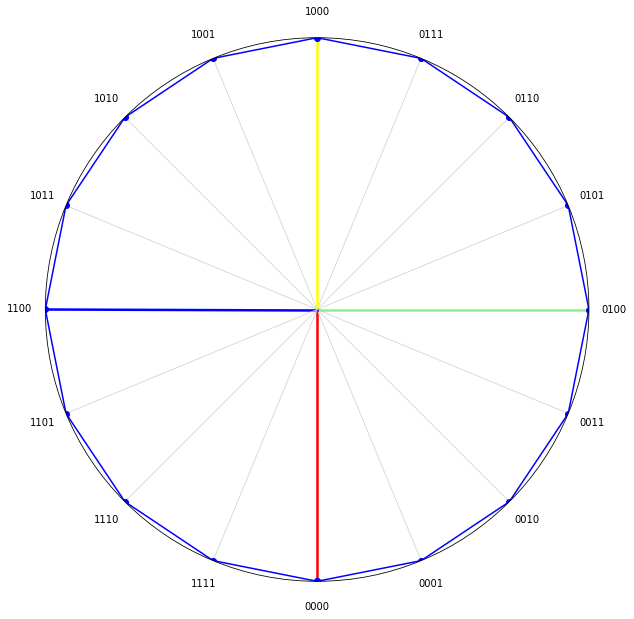
\includegraphics[width=0.9\linewidth]{img/posit4xRing.png}
  \captionof{figure}{Projection of a \posit{4}{x}}
  \label{fig:posit4xRing}
\end{minipage}%
\begin{minipage}{.5\textwidth}
  \centering
  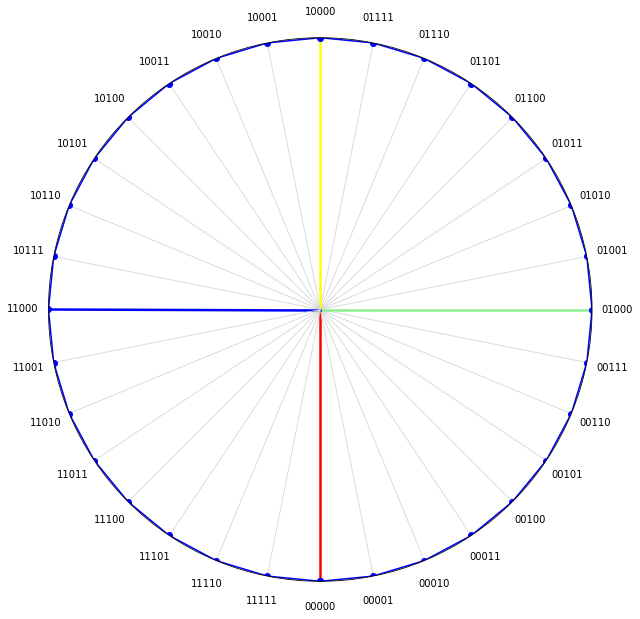
\includegraphics[width=0.9\linewidth]{img/posit5ring.png}
  \captionof{figure}{Projection of a \posit{5}{x}}
  \label{fig:posit5xRing}
\end{minipage}
\end{figure}

Figures \ref{fig:posit4xRing} and \ref{fig:posit5xRing} show the ring plot for a \posit{4}{x} and a \posit{5}{x} (exponent size is not relevant for the shape of the ring plot). The axis highlighted in \textbf{\textcolor{red}{red}} represents the real value $0$. The axis highlighted in \textbf{\textcolor{lightgreen}{green}} represents the real value $1$ and closes the first quarter of posit representations. The axis highlighted in \textbf{\textcolor{yellow}{yellow}} represents $\pm \infty$ (or \texttt{NaR}, depending on the configuration); this axis closes the quadrant where real values represented by posits are positive (note that also the integer representing the posit is positive). The axis highlighted in \textbf{\textcolor{blue}{blue}} represents the value $-1$. Note that these 4 points are fixed at south, west, north and east for any posit configuration. Indeed, they corresponds to the following posit integer representations: \textcolor{red}{0}, \textcolor{lightgreen}{$2^{nbits-2}$}, \textcolor{yellow}{$2^{nbits - 1}$} and \textcolor{blue}{$3 \cdot 2^{nbits-2}$}.

According to these two values, we can explicate the rounding, overflow and underflow behaviour of the format:
\begin{itemize}
    \item If we are trying to represent a real value $0 < r < \text{minposit}$ we will saturate it to $minposit$ to avoid underflow to $0$.
    \item If we are trying to represent a real value $r > \text{maxposit} $ we will saturate it to $\text{maxposit}$.
    \item If we are trying to represent a real value that lies between two exact posits, we need to round it to the nearest value (in terms of $L^2$ distance).
\end{itemize}




\section{A focus on decimal accuracy}

As we said in the previous Section, since the posit format has a variable length field for the fraction, the decimal accuracy (i.e. the number of allocated fraction bits for a given number) varies across the posit domain.

In particular, the fraction field depends on the length of the regime and exponent fields; given a \posit{nbits}{esbits} the regime field can have a length 
\begin{equation}
l_r \in [2,\text{nbits}-2]
\end{equation}
Consequently, the exponent field can have a length 
\begin{equation}
l_e = \text{min}(\text{esbits},\text{nbits}-2-l_r)
\end{equation}

Finally, the fraction field can have a length:
\begin{equation}\label{eqn:fracFieldLength}
l_f = \text{nbits} - 2 - l_r - l_e
\end{equation}

Looking at the fraction field length in \eqref{eqn:fracFieldLength}, we see that, when the regime value $k$ (see \eqref{eqn:regimeValue}) increases in absolute value, the fraction field length decreases; this means that, when numbers are very large or very small (in absolute value) - i.e. numbers with large positive or negative regime values - the fraction field has fewer bits available for allocation. On the other hand, when the regime value decreases (in absolute value), the fraction field length increase; this means that, when numbers are very close to $1$ (in absolute value), the fraction field has more bits available for allocation. 

Having more bits available for the fraction means that we can represent more precisely numbers after the decimal dot.

\begin{figure}
    \centering
    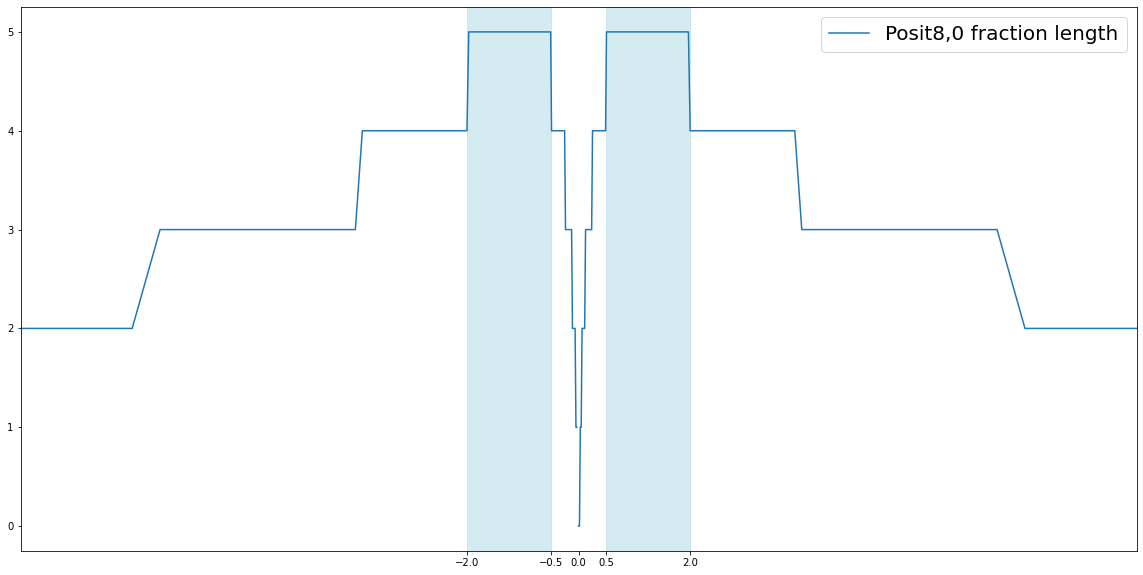
\includegraphics[width=\linewidth]{img/posit80fractionsWithZoom.png}
    \caption{\posit{8}{0} fraction length across the domain}
    \label{fig:posit80Fractions}
\end{figure}

Figure \ref{fig:posit80Fractions} shows this behaviour across the domain for a \posit{8}{0} configuration. In the plot we can see the region highlighted with the highest number of fraction bits with the associated real values $r \in [-1.9785,-0.5] \cup [0.5,1.9785]$


\begin{figure}
    \centering
    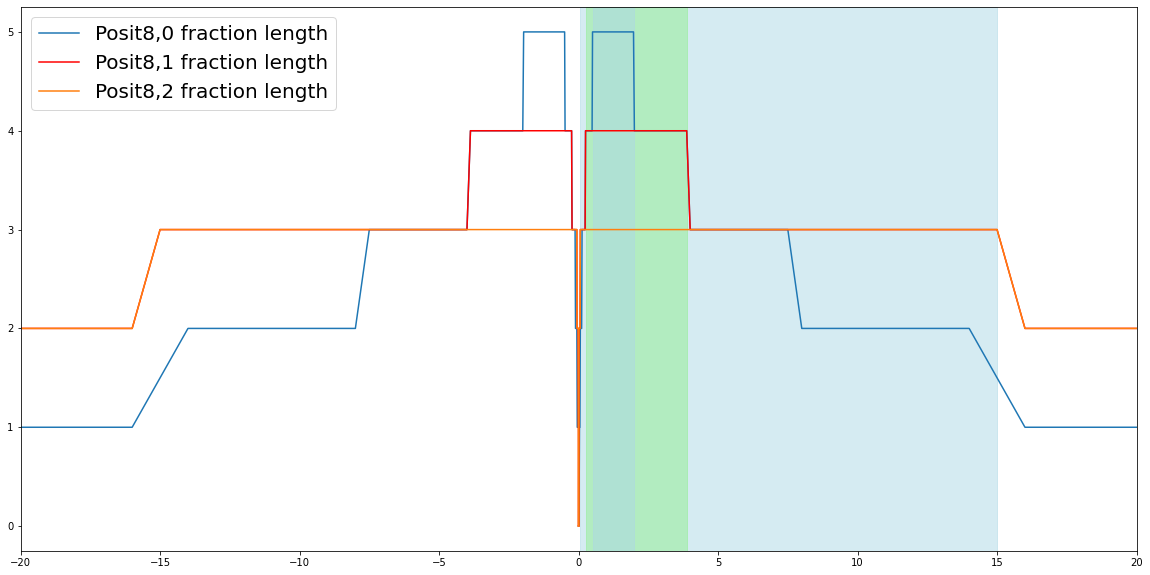
\includegraphics[width=\linewidth]{img/posit8xFractions.png}
    \caption{\posit{8}{x} fraction length comparison}
    \label{fig:posit8xFractions}
\end{figure}

Figure \ref{fig:posit8xFractions} shows the comparison of the fraction length between different configurations \posit{8}{[0,1,2]}. Obviously, if we allocate more bits for the exponent we are furtherly restricting the fraction bits, hence the different fraction bit lengths of the three configurations. However, with more exponent bits the range of maximum fraction bits is larger, despite containing the same number of distinct representations. This reflects on the format having a denser area of very high precision representation that thins out when we increase the exponent bits. 

We can generalize the range where the fraction has the highest amount of bits allocated:
\begin{equation}\label{eqn:highestFractionBits}
    \left [ \frac{1}{\text{useed}} , \text{useed} \right ) = \left [ \frac{1}{2^{2^{\text{esbits}}}}, 2^{2^{\text{esbits}}} \right )
\end{equation}

As we can see from Figure \ref{fig:posit8xFractions}, this range is always symmetric around the y-axis, so we have the two following ranges:
\begin{equation}\label{eqn:highestFractionBitsFull}
 \left ] -\text{useed}, -\frac{1}{\text{useed}} \right )  ; \left [ \frac{1}{\text{useed}} , \text{useed} \right )
\end{equation}

Note that both in \eqref{eqn:highestFractionBits} and \eqref{eqn:highestFractionBitsFull}, the sets are open from the side of $\text{useed}$. This is because, by design, the last positive posit with the highest number of fraction bits is the one immediately preceding the posit representing $\text{useed}$.

\begin{table}
\caption{Ranges of the maximum fraction bits numbers for different posit configurations}
\label{tab:positXxMaxFractionRanges}
\centering
\begin{tabular}{c|rl}
Configuration               & Negative range                    & Positive range             \\ \hline
 \posit{8}{0}               & $[-1.96875, -0.5]$                  & $[0.5, 1.96875]$         \\
 \posit{8}{1}               & $[-3.875, -0.25] $                  & $[0.25, 3.875]$       \\
 \posit{8}{2}               & $[-15.0, -0.0625]   $               & $[0.0625, 15.0]$         \\
 \posit{16}{0}              & $[-1.9998779296875, -0.5]$          & $[0.5, 1.9998779296875]$ \\
 \posit{16}{1}              & $[-3.99951171875, -0.25] $          & $[0.25, 3.99951171875]$  \\
 \posit{16}{2}              & $[-15.99609375, -0.0625]$           & $[0.0625, 15.99609375]$ 
\end{tabular}
\end{table}

Table \ref{tab:positXxMaxFractionRanges} summarizes the ranges of maximum fraction length for different posit configurations. As we can see the range span depends on the exponent bits (\textit{esbits}), while the decimal accuracy of the range bounds depends on the total number of bits (\textit{nbits}).

Another useful concept to understand the behaviour of posits across their domain is the \textit{resolution}. Given a pair of consecutive posit representations $p_1, p_2 = p_1 + 1; p_1, p_2 \in \mathbb{Z}$, we define resolution the value:
\begin{equation}\label{eqn:positResolution}
    \overline{r} = r_2 - r_1
\end{equation}

Where $r_1,r_2 \in \mathbb{R}$ are the real values associated, respectively, to $p_1, p_2$. Resolution represents the inverse of \textit{density} of a given format in a given range of numbers: the lower the resolution, the closer the real values associated with two consecutive representations.

\begin{figure}
    \centering
    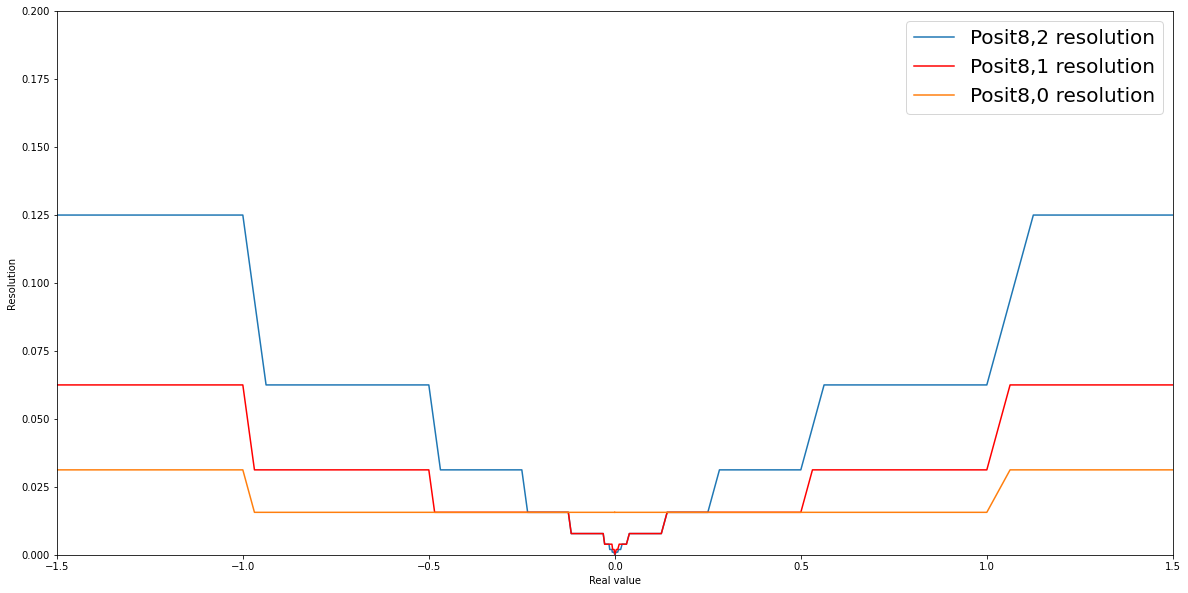
\includegraphics[width=\linewidth]{img/posit8xResolutions.png}
    \caption{\posit{8}{\{0,1,2\}} resolution across a portion of domain}
    \label{fig:posit8xResolutions}
\end{figure}

Figure \ref{fig:posit8xResolutions} shows the plot of $\overline{r}$ as function of $p_1$ for three configurations of \posit{8}{x}. As we can see, the \textit{resolution} decreases when approaching the value $0$ on the x-axis. Furthermore, the value of $\overline{r}$ is always smaller when using fewer exponent bits, this means that real numbers represented by successive posits are closer if compared to other posit configurations with a higher number of bits. As reported, the configurations for \posit{x}{0} have a flat resolution in the range $\left [ -1, 1 \right]$. This behaviour will be deeply analyzed in Section \ref{sec:Posit0bitExponent}.

\section{Posit and IEEE binary interoperability}\label{sec:fir}

One of the core concepts we deal with when bringing together the posit and the floating point domains is the interoperability between the two worlds. This means that we need to have two functions $f,g$ such that, given a set of Posits $\mathbb{P}$ and a set of floating point numbers $\mathbb{F}$:
\begin{equation}
    f: \mathbb{P} \xrightarrow[]{} \mathbb{F}
\end{equation}
\begin{equation}
    g: \mathbb{F} \xrightarrow[]{} \mathbb{P}
\end{equation}
Note that these two functions must be independent of the posit configuration \\\posit{nbits}{esbits} and the floating point type.
We introduce a \textit{float intermediate representation} (FIR) - i.e. a contact interface between any posit and any float configuration. Similarly to an IEEE binary, an FIR interface has three fixed-length fields:
\begin{itemize}
    \item sign $s_f$ on $1$ bit
    \item exponent $e_f$ on $\text{E}_f$ bits
    \item fraction $f_f$ on $\text{F}_f$ bits
\end{itemize}
Differently from the IEEE binary formats, the exponent here is a \textit{pure} one, without any offset applied. This means that the correspondent real value $r$ is:
\begin{equation}\label{eqn:firEquation}
    r = (-1)^{s_f} \cdot 2^{e_f} \cdot \left(1 + \frac{f_f}{2^{F_f}} \right)
\end{equation}
This interface allows us to decouple any posit configuration from any floating point configuration for conversion. Instead, we define another couple of functions $f_{fir}, 
g_{fir}$ that converts a posit into the FIR space and vice-versa.
On the other side, we need to provide another couple of functions for conversion between FIR and floating point space.
We can now characterize the two functions $f_{fir}, g_{fir}$ comparing Equations \eqref{eqn:positRealValue} and \eqref{eqn:firEquation}. If we take the general case from \eqref{eqn:positRealValue} and we expand the $useed$ term with \eqref{eqn:useed} we obtain:
\begin{equation}\label{eqn:positRealExpanded}
    r = (-1)^s_p \cdot 2^{2^{esbits} \cdot k + e_p} \cdot \left ( 1+ \frac{f_p}{2^{F_p}} \right)
\end{equation}
If we compare Equation \eqref{eqn:positRealExpanded} and \eqref{eqn:firEquation} we can impose equality on the three terms of the multiplication. The sign equality is straightforward: the sign of the number in FIR format must match the posit one.
If we are converting from posit to FIR, we can obtain the exponent $e_f$ as:
\begin{equation}
    e_f = 2^{esbits} \cdot k + e_p
\end{equation}
If we are converting the other way we can obtain $k$ and $e_p$ using modular arithmetic in base $2$: 
\begin{equation}
    k = \left\lfloor \frac{e_f}{2^{esbits}} \right\rfloor
\end{equation},
\begin{equation}
    e_p = e_f\ \mathbf{mod}\ 2^{esbits}
\end{equation},
where $\mathbf{mod}$ is the remainder.
For the fraction we need to impose the equality:
\begin{equation}\label{eqn:fractionalPartEquivalence}
    \frac{f_f}{2^{F_f}} = \frac{f_p}{2^{F_p}}
\end{equation}
Then we can solve for $f_f$ as:
\begin{equation}
    f_f = f_p \cdot 2^{F_f - F_p}
\end{equation}
and we can solve for $f_p$ as:
\begin{equation}
    f_p = f_f \cdot 2^{F_p - F_f}
\end{equation}
Note that, depending on the fraction sizes, the operation may result in loss of information, when we shrink a fraction with more bits to one with fewer bits.  Therefore, we need to take into account the bits we are discarding to eventually round the destination format according to their value.

So far, we have covered the conversion between FIR and posit numbers. The conversion between FIR and IEEE binary (or whichever floating point format) is similar, if not simpler.
Let us consider the IEEE binary32 conversion from/to a given FIR format. 
The exponent $e_{b32}$ of a binary32 number must be offset by $127$ during the transition between the two formats. Therefore, given $e_f$ the FIR exponent, we obtain:
\begin{equation}
    e_{b32} = e_f + 127
\end{equation}
On the other hand:
\begin{equation}
    e_{f} = e_{b32} - 127
\end{equation}
The fractional part can be handled as in \eqref{eqn:fractionalPartEquivalence}. Note that, differently from posit numbers, when the exponent is $0$, the fractional part of a binary32 needs to be interpreted without the leading $1.$ (i.e. the number must be considered as a subnormal).
Note that, the approach of using an intermediate representation can be used between whichever formats for real numbers that can be represented in the sign, exponent and fraction format.


\section{Generalized posits}

As seen in Figures \ref{fig:posit80Fractions} and \ref{fig:posit8xFractions}, the regime length has a sensible impact on the number of fraction bits we can use across the domain. Such length can change to the point that we do not have sufficient decimal accuracy (depending on the application) in a given range of numbers. 
An ideal approach would be to impose an upper limit to the regime length such that we can be sure that we will always reserve at least some bits for the fraction.
In \cite{9151086}, the authors propose a new way to characterize posit numbers. Additionally to the \textit{nbits}  and \textit{esbits} parameters, there are two (mutually exclusive) new parameters that control the dynamic range:
\begin{itemize}
    \item $K_b$: a regime bias 
    \item $rs$: a limit on the regime length
\end{itemize}
This results in having the maximum posit value shifted at:
\begin{equation}
    2^{2^{esbits} \cdot (k-K_b)}
\end{equation}
if using the $K_b$ parameter, or if we use the $rs$ parameter:
\begin{equation}
    2^{2^{esbits} \cdot rs} \cdot (1 - 2^{es - t - 1})
\end{equation}
where $ t = n - rs - 1$.


\section{A special case: 0-bit exponent}\label{sec:Posit0bitExponent}

In this section we focus on the posit format when configured with 0 exponent bits (i.e. \posit{x}{0}), also referring to our work in \cite{coco2020sensors}. In general, the operations presented in this section allows for their computation without the need of decoding the posit, thus simplyfing the software (or hardware) involved in their elaboration. These operators introduce very interesting properties and results: (i) faster evaluation than the exact counterpart with a negligible accuracy degradation; (ii) enabling an efficient ALU emulation of a number of Posits operations; (iii) enabling the possibility to vectorize operations n Posits, using existing ALU vectorized operations (such as the Scalable Vector Extension of ARM CPUs or Advanced Vector Extensions on Intel CPUs). While using 0 bit for the exponent reduces the dynamic range of the posit (see Equation \eqref{eqn:useed}), it allows for an higher density of representation when approaching \texttt{minposit} (see Figures \ref{fig:posit8xResolutions} and \ref{fig:posit8xDistributions}). Given these properties, it is worth to deepen on the behaviour of \posit{n}{0}.

If we impose $esbits = 0$ - that means also $es = 0$ - in \eqref{eqn:positRealValue}, we get:
\begin{equation}\label{eqn:positRealValueExp0}
    (-1)^s \cdot \text{2}^{k} \cdot \left ( 1+ \frac{f}{2^F} \right)
\end{equation}


\begin{figure}
    \centering
    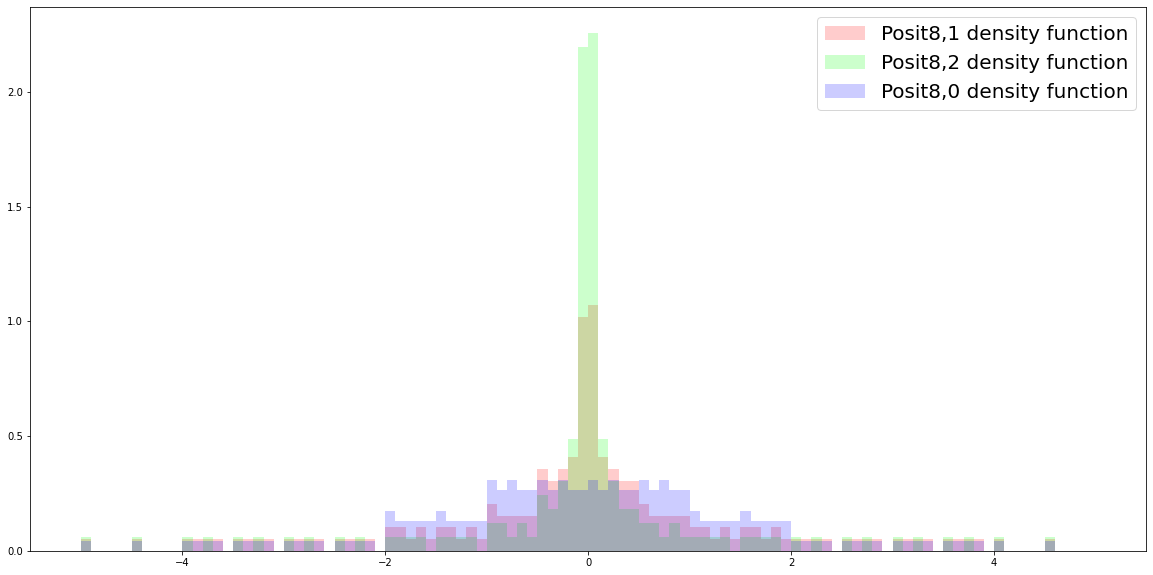
\includegraphics[width=\linewidth]{img/posit8xDensities.png}
    \caption{\posit{8}{x} density distribution around $0$.}
    \label{fig:posit8xDistributions}
\end{figure}

since $useed = 2^{2^0} = 2$. Having no exponent bits results in the behaviour shown in Figures \ref{fig:posit8xFractions} and \ref{fig:posit8xDistributions}. In particular, looking at Figure \ref{fig:posit8xDistributions}, the density distribution of a \posit{8}{0} tends to decay slower when moving away from the origin, thus having a better coverage in the range $[-useed,useed]$ when compared to posits with more exponent bits. This can be also seen in Figure \ref{fig:posit8xResolutions}, where the resolution of \posit{8}{0} is constant in $[-1,1]$ while the resolution of the other two posits increases also in this range. 
As we mentioned in the previous section, a 0-exponent bit posit in the range $[-1,1]$ has the property of having a constant resolution. 
We know that the fraction length $F_p$ depends on the regime length $l$ and, as a consequence, on the regime value $k$. In the range $[-1,1]$, we also know that the regime value is always $k \leq 0$, with the equality holding for posit representing real values of $\pm 1$. This means that in this region, the associated length (excluding the regime stop bit) is $l = - k$. Therefore, the fraction length $F$ can be written as $nbits - l - 2$, where $2$ includes the sign-bit and regime stop bit. We can rewrite \eqref{eqn:positRealValueExp0} as:
\begin{equation*}
    (-1)^s \cdot 2^k \cdot \left ( 1 + \frac{f_p}{2^{nbits + k - 2}} \right )
\end{equation*}
If we distribute the term $2^k$ inside the parenthesis we obtain:
\begin{equation*}
    (-1)^s \cdot \left ( 2^k + \frac{f_p\cdot 2^2}{2^{nbits}} \right )
\end{equation*}

\begin{equation*}
    (-1)^s \cdot \left ( \frac{2^{k+nbits}}{2^{nbits}} + \frac{f_p\cdot 2^2}{2^{nbits}} \right )
\end{equation*}

\begin{equation*}
    (-1)^s \cdot \left ( \frac{2^{k+nbits} + f_p\cdot 2^2}{2^{nbits}} \right )
\end{equation*}

\begin{equation*}
    (-1)^s \cdot \left ( \frac{2^2 \cdot (2^{k+ nbits - 2} + f_p)}{2^{nbits}} \right )
\end{equation*}

\begin{equation}\label{eqn:posit0exponentInUnitaryRange}
    (-1)^s \cdot \left ( \frac{2^2 \cdot (2^{F_p} + f_p)}{2^{nbits}} \right )
\end{equation}
Note that the value $2^{F_p} + f_p$ represents exactly the last $F_p + 1$ bits of the posit, since the fraction numerator $f_p$ is exactly $F_p$ bits long. Moreover, since the regime bits are in the format $000 \cdots 01$ and $2^{F_p}$ represents exactly the $1$ stopping bit, the integer $P$ representing the posit is exactly:
\begin{equation}\label{eqn:posit0expUnitary}
    P = 2^{F_p} + f_p
\end{equation}
Let us compare \eqref{eqn:posit0exponentInUnitaryRange} with \eqref{eqn:fixed2real}. In order to impose the equality between the two equations, $2^2 \cdot ( 2^{F_p} + f_p )$ must be equal to $f$ and $nbits$ must be equal to $F$ in \eqref{eqn:fixed2real}. Then, the integral part $i$ must be 0, since we are in the unitary range.
Therefore,  a \posit{x}{0} in the range $[-1,1]$ is equivalent to a fixed-point on $2\cdot x$ bits with a fractional part equal to $2^2 \cdot ( 2^{F_p} + f_p )$.
In practice, given a \posit{x}{0} we can just shift the posit representation two places left (hence the $2^2$ in \eqref{eqn:posit0exponentInUnitaryRange}) to obtain the fractional part of the correspondent fixed point number without any rounding.


\subsection{Fast arithmetic operation implementation
}\label{subsec:fastArithOps}

A format with $0$ exponent bits paves the way to implement several arithmetic operations in a way that does not require decoding of the posit itself, with the risk of introducing an approximation.
Hereafter, we will present the mathematical formulation of several functions, while in Section \ref{sec:cppPositCore} we will evaluate the performance and approximation error of such operations.

\subsubsection{Inverse}
 
Let us start with the reciprocating formulation:
\begin{equation}
    y = \frac{1}{x}
\end{equation}
Firstly, we need to distinguish the formulations shown in \eqref{eqn:posit0exponentInUnitaryRange} from the range  $]-\infty,-1] \cup [1,\infty[$. When in this range, the regime value is always $k \geq 0$ ,  hence $l = k + 1$. This means that the number of bits for the fraction is $F = nbits - k - 3$. We can then write two different formulation for the real value associated to a \posit{x}{0}, where $r^- \in (-1,1)$ and $r^+ \in (-\infty, -1] \cup [1,\infty)$:
\begin{equation}
   r^- =  (-1)^s \cdot 2^k \cdot \left ( 1 + \frac{f_p}{2^{nbits + k - 2}} \right )
\end{equation},

\begin{equation}
   r^+ = (-1)^s \cdot 2^k \cdot \left ( 1 + \frac{f_p}{2^{nbits - k - 3}} \right )
\end{equation}
\begin{figure}
    \centering
    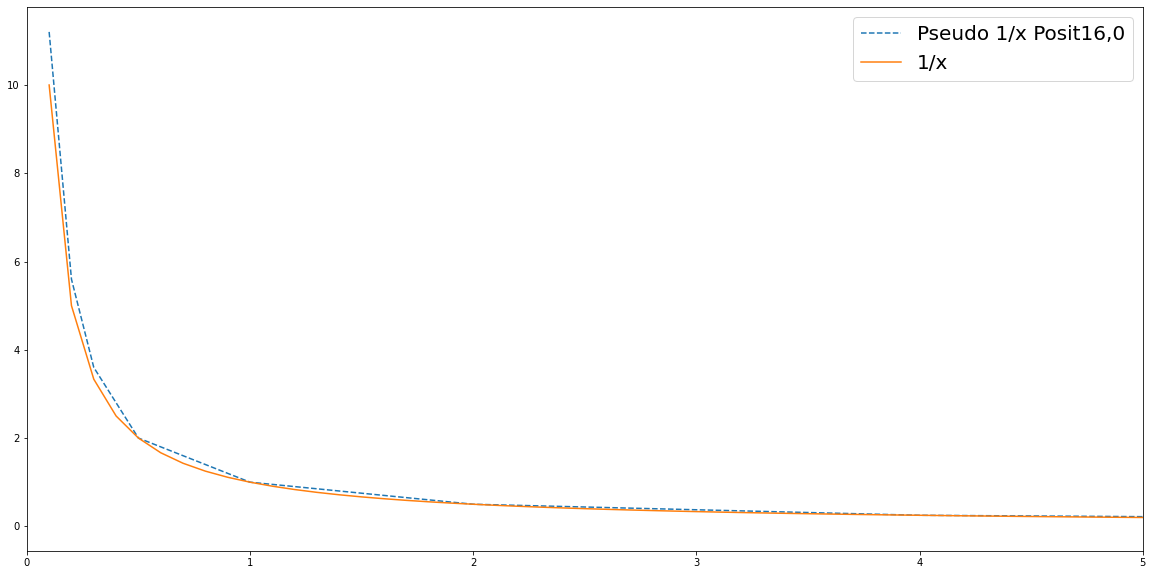
\includegraphics[width=\linewidth]{img/invPosit160.png}
    \caption{Comparison between exact inverse and decoding-free inverse for \posit{16}{0}}
    \label{fig:invPosit160}
\end{figure}
Now, let $x, y = \frac{1}{x}$ be two posits encoded with, respectively $s_x,k_x, f_x$ and $s_y = s_x, k_y, f_y$. Since there is an inversion, if $x \in [-1,1]$ then $y \in (-\infty, -1] \cup [1,\infty)$ (or vice-versa). We want to express $x \cdot y \sim 1$ using the posit representation of a real:
\begin{equation}\label{eqn:positx0prodInverse}
    x \cdot y = 2^{k_x+k_y} \cdot \left[ \left (1 + \frac{f_x}{2^{2^{nbits + k_x - 2}}} \right ) \cdot \left (1 + \frac{f_y}{2^{2^{nbits - k_y - 3}}} \right ) \right] \simeq 1
\end{equation}

We need to distinguish two cases:
\begin{itemize}
    \item[a)]$f_x = 0$, i.e. x is a pure exponential number and has an exact inversion in the posit space representation
    \item[b)] $f_x \neq 0$, i.e. x has also a fractional part and it has not an exact inversion in the posit space representation
\end{itemize}
Indicating with $P$ the integer representing the posit number, we can test the case as follows (i.e. the number is a pure exponential one if): 
\begin{equation}
    P\ \mathbf{and}\ (P - 1) = 0
\end{equation}.

\paragraph{Case a)} When in case a), we know that $k_y = -k_x$ (from inversion of \eqref{eqn:positRealValueExp0}). If we substitute this in \eqref{eqn:positx0prodInverse} we obtain:
\begin{equation}
    x \cdot y = 2^{0} \cdot \left[ \left (1 + \frac{f_x}{2^{2^{nbits + k_x - 2}}} \right ) \cdot \left (1 + \frac{f_y}{2^{2^{nbits + k_x - 3}}} \right ) \right] \simeq 1
\end{equation}
We then develop the product inside the square brackets, discarding the product between the fraction themselves, introducing no approximation since $f_x = f_y = 0$:
\begin{equation}
    x \cdot y = 2^{0} \cdot \left[ 1 + \frac{f_x}{2^{2^{nbits + k_x - 2}}}  + \frac{f_y}{2^{2^{nbits + k_x - 3}}} \right] \simeq 1
\end{equation}
Since the number must be equal to $1$, we impose the fractional part to be $0$, therefore:
\begin{equation}
    f_x + 2\cdot f_y = 0
\end{equation}
Since we already know that $f_x$ and $f_y$ are $0$, this holds by construction. 

Therefore, in this case the only transformation needed is $k_y = -k_x$. Since $k_x \leq 0$, changing the sign reflects on the length being increased by $1$. This means that the regime bits must be flipped and another bit of the same value must be appended to the regime. Since $f_x = 0$, if we invert it and add $1$ we get a bit set on the F-th least significant bit - i.e. on the former regime stop-bit. Wrapping everything up, we can obtain the inverse of $x$ with this expression, being $X$,$Y$ the integer numbers representing the posits:
\begin{equation}
    Y = X\ \mathbf{xor}\ (2^{nbits - 1} - 1) + 1
\end{equation}

\paragraph{Case b)} When in case b), $k_y = -k_x - 1$ (again from the inversion of \eqref{eqn:positRealValueExp0}). If we substitute this again \eqref{eqn:positx0prodInverse} we obtain:
\begin{equation}
    x \cdot y = 2^{-1} \cdot \left[ \left (1 + \frac{f_x}{2^{2^{nbits + k_x - 2}}} \right ) \cdot \left (1 + \frac{f_y}{2^{2^{nbits + k_x - 2}}} \right ) \right] \simeq 1
\end{equation}
Again, we develop the product inside square brackets, discarding the fraction product, now introducing an approximation:
\begin{equation}
    x \cdot y = 2^{-1} \cdot \left[ 1 + \frac{f_x}{2^{2^{nbits + k_x - 2}}}  + \frac{f_y}{2^{2^{nbits + k_x - 2}}} \right] \simeq 1
\end{equation}
Since the product must be $\sim 1$, we solve by $f_y$, obtaining:
\begin{equation}
\left\{\begin{matrix}
k_y = -k_x - 1 \\
f_y = 2^{F_x} - f_x
\end{matrix}\right.
\end{equation}

When changing the sign of $k_x$, we are acting like in case a), increasing the length of the regime by $1$ and changing its sign. However, now we also subtract $1$ from it, thus maintaining the regime length identical. This equals just flipping the regime bits.  For the fraction, we are subtracting an integer on $F_x$ bits - that is $f_x$ - from the value $2^F{_x}$. This again is equal to flipping $f_x$ bits and adding $1$. Since the case of $f_x = 0$ is not possible in b), this operation will never overflow $F_x$ bits, hence we can flip all the posit bits (excluding the sign) and add $1$. Wrapping everything up, let $X,Y$ be the integers representing the posits:

\begin{equation}
    Y = X\ \mathbf{xor}\ (2^{nbits - 1} - 1) + 1
\end{equation}
We obtained that, in both cases a) and b), the formulation for the inversion is the same, so we can fuse the two into one. However, the second case introduces, inevitably, an approximation since we discarded the product between fractions inside the square brackets.

\subsubsection{$\mathbf{2\cdot x}$ and $\mathbf{x/2}$}

Let us proceed with the $y = 2\cdot x$ operation. For this operation we need to distinguish three ranges for the real value $r$:


\begin{itemize}
    \item[a)] $r \in (-0.5,0] \cup [0,0.5) \xrightarrow{} 2\cdot r \in (-1,1)$
    \item[b)] $r \in (-1,-0.5] \cup [0.5,1) \xrightarrow{} 2\cdot r \in (-2,-1] \cup [1,2) $
    \item[c)] $r \in (-\infty, -1] \cup [1, \infty)  \xrightarrow{} 2\cdot r \in (-\infty, -2] \cup [2, \infty)$
\end{itemize}
Regardless of the case we are in, we can write the following expression for the operation $y = 2 \cdot x$:

\begin{equation}
    y = 2 \cdot x = (-1)^{s_x} \cdot 2^{k_x + 1} \cdot \left(1 + \frac{f_x}{2^{F_x}} \right) 
\end{equation}
This means that, for all the cases, $k_y = k_x + 1$
For symmetry, we can focus only on the positive quadrant of the posit ring. The values $0.5,1,2$ are, respectively, represented by the integers $2^{nbits - 3}, 2^{nbits - 2}, 2^{nbits - 2} + 2^{nbits - 3}$.

\paragraph{Case a)} When $x \in [0,0.5)$ we know that $k_x \leq 0$, therefore $l_x = -k_x$. We also know that $y = 2\cdot x = \in [0,1)$, therefore $k_y \leq 0$ and $l_y = -k_y$. If we substitute the equivalence  $k_y = k_x + 1$ we obtain:
\begin{equation}
    l_y = - (k_x + 1) = l_x - 1
\end{equation}
In case a), we know that both $k_x, k_y$ will be in the form $000 \dots 01$. In particular, after multiplying by $2$, the regime length of $y$ will be shorter by 1. This corresponds to shifting the posit one position to the left. Since we are operating on positive numbers, we are guaranteed that the sign is preserved. Let $X,Y$ be the integer for the posits that represent $x,y$:
\begin{equation}
    Y = \mathbf{lls} (X,1) = 2 \cdot X
\end{equation}
where $\mathbf{lls}(X,N)$ is the logical left shift of the integer $X$ of $N$ positions.
\paragraph{Case b)} When $x \in [0.5,1)$ we know that $k_x \leq 0$ again. Hence, $l_x = -k_x$. In this case, $y = 2\cdot x \in [1,2)$, thus $k_y \geq 0$ and $l_y = k_x + 2$. Substituting the equivalence $k_y = k_x + 1$ we obtain:
\begin{equation}
    l_y = 2 - l_x
\end{equation}
Note that when $esbits = 0$, the range expressed in \eqref{eqn:highestFractionBits} is $[0.5,2)$ This means that $\forall x \in [0.5,2), l_x = 1$ and, as a consequence, we will always have $l_y = 2 - l_x = 1$. While $l_x = 1$ for a negative $k_x = -1$, $l_y = 1$ for a positive $k_y = 1$. This means that we need to flip the regime bits. Since we are in the region with the minimum number of regime bits (i.e. 2 regime bits, including the stopping bit), we just need to flip the 2 most significant bits (ignoring the sign). Let $X,Y$ be the integer for the posits that represent $x,y$:
\begin{equation}
    Y = X\ \mathbf{xor}\ (2^{nbits - 2} + 2^{nbits - 3})
\end{equation}


\paragraph{Case c)} When $x \in [1,\infty)$ we know that both $k_x \geq 0$ and $k_y \geq 0$. Therefore, $l_x = k_x + 1$ and $l_y = k_y + 1$. Substituting the equivalence $k_y = k_x + 1$ we obtain:
\begin{equation}
    l_y = l_x + 1
\end{equation}
In this case, the regime bits are in the format $111 \cdots 10$. When we multiply by two we are increasing the regime and the regime length by $1$. This means that we need to put a single bit set in front of the regime and then shift the posit to the right (possibly discarding the fraction least significant bit). Let $X,Y$ be the integer for the posits that represent $x,y$:
\begin{equation}
    Y = (X\ \mathbf{or}\ 2^{nbits - 1}) \cdot 2^{-1}
\end{equation}
Note that we can elaborate in the same way for the $x/2$ operation: this case is omitted because it is symmetrical to the previous one and symmetrical would be the results obtained. 



\subsubsection{Unitary complement: $\mathbf{1-x}$}

Suppose we are in the $[0,1]$ range and we want to perform the \textit{unitary complement} of a number $x$, that is:
\begin{equation}
    y = 1 - x    
\end{equation}
As seen before in \eqref{eqn:posit0expUnitary}, in the unitary range the posit integer $P = 2^{F_p} + f_p$. 
To derive an expression for this complement operation we can write $x + y = 1$ and expand the terms:
\begin{equation}
    2^{k_x} \cdot \left(1 + \frac{f_x}{2^{F_x}} \right) + 2^{k_y} \cdot \left(1 + \frac{f_y}{2^{F_y}} \right) = 1
\end{equation}
When in the unitary range we already know that $k \leq 1$ and $F = nbits - 2 + k$ for both $x$ and $y$. If we substitute this in both the terms of the addition we obtain:
\begin{equation}
    2^{k_x} + \ 2^{k_y} + \frac{f_x + f_y}{2^{nbits - 2}} = 1
\end{equation}
We multiply both sides by $2^{nbits - 2}$ obtaining:
\begin{equation}
    2^{F_x} + 2^{F_y} + f_x + f_y = 2^{nbits - 2}
\end{equation}
We then apply  \eqref{eqn:posit0expUnitary}, obtaining the expression needed to compute $y = 1 - x$:
\begin{equation}
    X + Y = 2^{nbits - 2} \xrightarrow{} Y = 2^{nbits - 2} - X
\end{equation}



\subsubsection{Sigmoid}
\begin{figure}
    \centering
    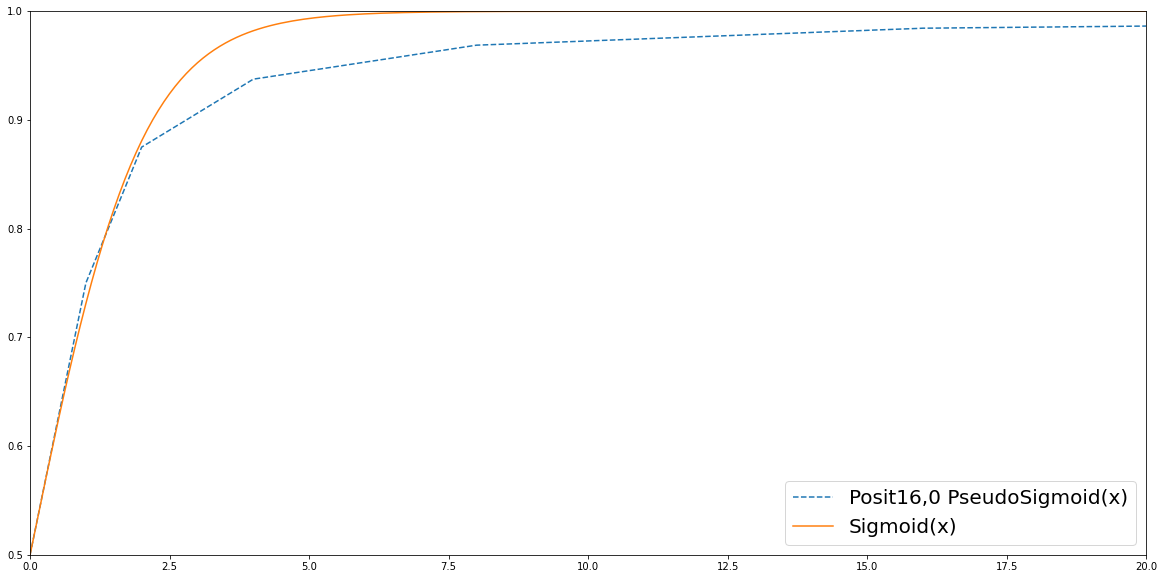
\includegraphics[width=\linewidth]{img/sigmoidPosit160.png}
    \caption{Actual sigmoid vs plot of the integer representation of a \posit{16}{0}}
    \label{fig:posit160Sigmoid}
\end{figure}

In \cite{gustafson2017beating}, John L. Gustafson et al. observed a particular property of the posit representation when plotting the integer value representing the posit and the correspondent real value.

The sigmoid curve is a very well-known activation function for neural networks:
\begin{equation}
    \mathbf{sigmoid}(x) = \frac{1}{1 + e^{-x}}
\end{equation}

If we look at Figure \ref{fig:posit160Sigmoid} we can see that the actual sigmoid curve is very similar to the curve obtained by plotting the value of the integer $P$ representing a posit $p$ for any correspondent real value $r$. However, the plot for $P$ must be scaled and translated to match the sigmoid output in $[0,1]$. The scaling and translation are performed as follows: let $\hat{S}(x)$ be the \textit{pseudo-sigmoid} shown in figure \ref{fig:posit160Sigmoid}, and $X$ the integer representing the posit associated to the real value $x$:
\begin{equation}
    \hat{S}(x) = \frac{X}{2^{nbits}} + \frac{1}{2}
\end{equation}

In \cite{gustafson2017beating} the authors reported another version of this transformation, obtaining the posit integer representation for the sigmoid output from the posit integer representation of its input. Let $Y$ be the integer posit representation for the sigmoid $\hat{S}(x)$ and $X$ the posit integer representation associated to the real value $x$:
\begin{equation}\label{eqn:pseudoSigmoidPosit0}
    Y = \left ( 2^{nbits - 2} + \frac{X}{2} \right ) \cdot \frac{1}{2}
\end{equation}
As pointed out in \cite{coco2020sensors}, the two expressions are equivalent.

\subsubsection{Hyperbolic tangent}

\begin{figure}
    \centering
    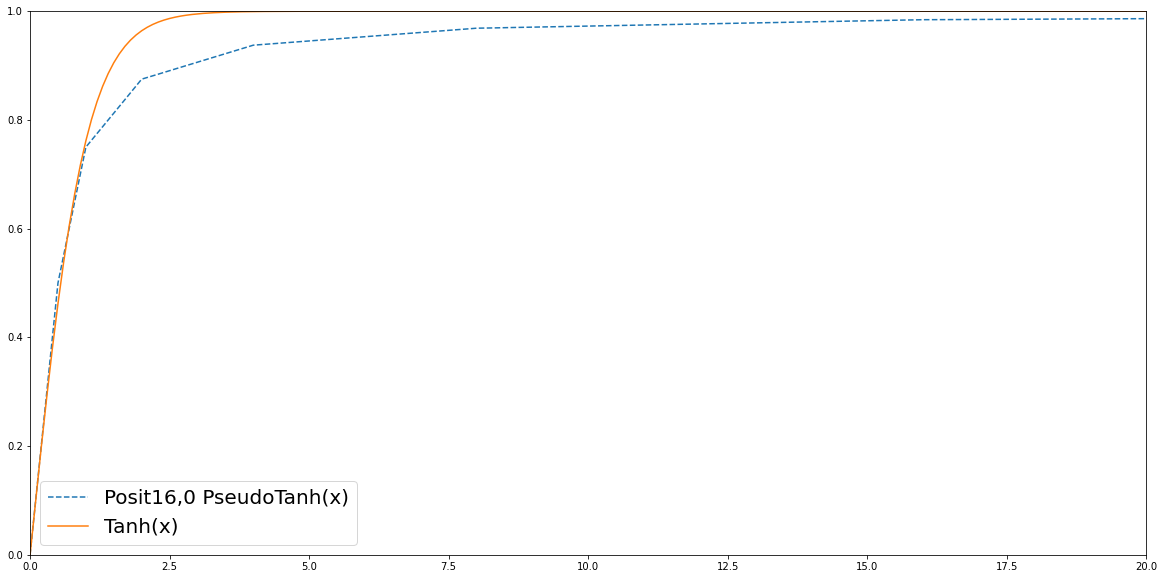
\includegraphics[width=\linewidth]{img/tanhPosit160.png}
    \caption{Hyperbolic tangent comparison between actual and pseudo version.}
    \label{fig:pseudoTanhPosit0}
\end{figure}
The hyperbolic tangent is another commonly used activation function in neural networks. Its expression is quite similar to the sigmoid:
\begin{equation}
    \mathbf{tanh}(x) = \frac{e^{2x}-1}{e^{2x}+1} 
\end{equation}
We can obtain this expression from the sigmoid by applying a scale and a transformation:
\begin{equation}
   \mathbf{tanh}(x) =  2 \cdot \mathbf{sigmoid}(2 \cdot x) - 1
\end{equation}
We can rework the previous expression as follows:
\begin{equation}
    \mathbf{tanh}(x) = - ( 1 - 2\cdot \mathbf{sigmoid}(2\cdot x))
\end{equation}
Suppose we only consider negative values for $x$ for symmetry. We know that the $2\cdot x$ operation can be done without decoding with \posit{x}{0}. Since we are dealing with negative numbers, the output of the sigmoid will be in $[0,1/2]$. Again, multiplying this number by $2$ can be done without decoding the posit and the output will be in $[0,1]$. Therefore, we can apply the $1-y$ operation without decoding the posit. Finally, we can change the sign with a 2's complement of the representation.
If we substitute the sigmoid with the pseudo-sigmoid seen in \eqref{eqn:pseudoSigmoidPosit0} we obtain a decoding-free \textit{pseudo hyperbolic tangent}.

\subsubsection{Extended Linear Unit}

\begin{figure}
    \centering
    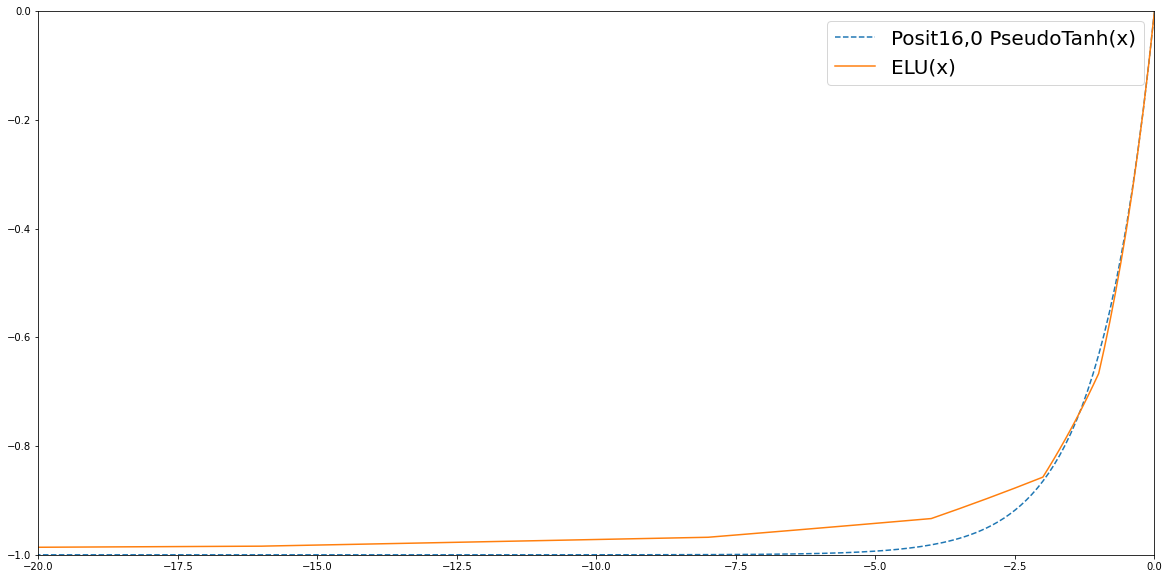
\includegraphics[width=\linewidth]{img/eluPosit160.png}
    \caption{ELU comparison between actual and pesudo version.}
    \label{fig:pseudoEluPosit0}
\end{figure}


The Extended Linear Unit (ELU) is another commonly used activation function in neural networks, mainly adopted to avoid vanishing gradients of S-shaped functions like a sigmoid and hyperbolic tangent.
The formulation of the ELU function is the following:

\begin{equation}
\mathbf{elu}(x)=\left\{\begin{matrix}
x & x \geq 0 \\
\alpha \cdot (e^x - 1) & x < 0  \\
\end{matrix}\right.
\end{equation}
The case for $x \geq 0$ is straightforward, so we focus on the $\alpha \cdot (e^x - 1)$ part. In particular, we consider the case where $\alpha = 1$, hence:
\begin{equation}
    \mathbf{elu}(x) = (e^x - 1) = 2 \cdot \left [ \frac{1}{2\cdot \mathbf{sigmoid}(-x)} - 1 \right]
\end{equation}

We can start from the sigmoid obtained before. We firstly negate the argument to have a sigmoid output in $[0.5,1]$. We can then invert without decoding obtaining an output in $[1,2]$. This output is divided by $2$, obtaining an output in $[0.5,1]$. We can apply the $1-y$ operation without decoding and then multiply everything by $2$ to obtain the final result in \eqref{eqn:sigm_twinvm1}.

\begin{align}
   \label{eqn:sigm_mx}\textnormal{sigmoid}(-x) = \frac{1}{1+e^{x}}  & \\
   \label{eqn:sigm_invx}1/\textnormal{sigmoid}(-x) = 1+e^x & \\
   \label{eqn:sigm_invtw}1/(2\cdot\textnormal{sigmoid}(-x)) = \frac{1+e^x}{2}& \\
   \label{eqn:sigm_invm1}1/(2\cdot\textnormal{sigmoid}(-x))-1 = \frac{1+e^x}{2} - 1 = \frac{e^x-1}{2} & \\
  \label{eqn:sigm_twinvm1}2\cdot[1/(2\cdot\textnormal{sigmoid}(-x))-1] = e^x -1&
\end{align}
If we substitute the sigmoid function with the pseud-sigmoid seen in \eqref{eqn:pseudoSigmoidPosit0} we obtain a decoding-free \textit{pseudo-ELU}.




\section{Arithmetic operations on posits}\label{sec:posit_ops}

In this section, we cover the different phases of binary operations between posits.

\subsection{Input conditioning and posit decoding}\label{input_conditioning_section}

Before the decoding of the posit operands, we make use of some logic meant to discriminate different cases of posit configurations. These are those cases where either one of the operands is $0$ (i.e. actual $0$ and NaR), or when the operation leads to straightforward output. All these cases can be reduced to simple ones that, similarly to the \textit{fast operations}, can be resolved without decoding the posit value. Handling these conditions upfront is important since it simplifies the rest of the logic for the operations.

\hypertarget{special_cases_link}{~}
\textit{special} and \textit{trivial} cases are those where, respectively:
\begin{itemize}
\item one of the inputs is \textit{special} (e.g. NaR or inf), which leads to a \textit{special} output
\item the output of a given operation is \textit{special} and this can be directly inferred from the inputs (e.g. division by zero).
\end{itemize}
If one of these cases is caught, the result is produced without decoding.
The possible combinations, for each of the four operation, are tabulated in \ref{table:table_posit_op_combination}, with a distinction between \textit{special} and \textit{trivial} cases.
Special cases are colored in \textcolor{red}{red}, and trivial are colored in \textcolor{orange}{orange}.
Each posit value can either be \textit{special}, i.e. $\in \{0$, \mbox{NaR}\}, or \textit{non-special}. 
In order to simplify the logic concerning addition/subtraction, we can already enforce an order between the inputs, so that $p_1$ and $p_2$ carry, respectively, the largest and smaller value (in absolute terms). At the same time, we reserve a flag indicating whether the sign of the two numbers is concordant or not. This observation will be used from now on to simplify the reasoning on the operational implementation.

\begin{table}
\begin{center}
\begin{tabular}{ cc }   % top level tables, with 2 columns
addition & subtraction \\
\begin{tabular}{||c c c | c||}
    \hline
    $p_1$ & op & $p_2$ & $p_{out}$ \\ [0.5ex]
    \hline\hline
    $0$ & $+$ & $0$ & \textcolor{red}{$0$} \\
    \hline
    $0$ & $+$ & NaR & \textcolor{red}{NaR} \\
    \hline
    $0$ & $+$ & $p_2$ & \textcolor{yellow}{$p_2$} \\ %%%% https://www.overleaf.com/learn/latex/Using_colours_in_LaTeX
    \hline
    NaR & $+$ & $0$ & \textcolor{red}{NaR} \\
    \hline
    NaR & $+$ & NaR & \textcolor{red}{NaR} \\
    \hline
    NaR & $+$ & $p_2$ & \textcolor{red}{NaR} \\
    \hline
    $p_1$ & $+$ & $0$ & \textcolor{yellow}{$p_1$} \\
    \hline
    $p_1$ & $+$ & NaR & \textcolor{red}{NaR} \\
    \hline
    $p_1$ & $+$ & $p_2$ & \textcolor{green}{$p_1 + p_2$} \\
    \hline %%% 2 more trivial cases
    $p_1$ & $+$ & $-p_1$ & \textcolor{yellow}{$0$} \\
    \hline
    $-p_2$ & $+$ & $p_2$ & \textcolor{yellow}{$0$} \\
    \hline
\end{tabular} &
\begin{tabular}{||c c c | c||}
    \hline
    $p_1$ & op & $p_2$ & $p_{out}$ \\ [0.5ex]
    \hline\hline
    $0$ & $-$ & $0$ & \textcolor{red}{$0$} \\
    \hline
    $0$ & $-$ & NaR & \textcolor{red}{NaR} \\
    \hline
    $0$ & $-$ & $p_2$ & \textcolor{yellow}{$-p_2$} \\ %%%% https://www.overleaf.com/learn/latex/Using_colours_in_LaTeX
    \hline
    NaR & $-$ & $0$ & \textcolor{red}{NaR} \\
    \hline
    NaR & $-$ & NaR & \textcolor{red}{NaR} \\
    \hline
    NaR & $-$ & $p_2$ & \textcolor{red}{NaR} \\
    \hline
    $p_1$ & $-$ & $0$ & \textcolor{yellow}{$p_1$} \\
    \hline
    $p_1$ & $-$ & NaR & \textcolor{red}{NaR} \\
    \hline
    $p_1$ & $-$ & $p_2$ & \textcolor{green}{$p_1 - p_2$} \\
    \hline %%% 2 more trivial cases
    $p_1$ & $-$ & $p_1$ & \textcolor{yellow}{$0$} \\
    \hline
    $p_2$ & $-$ & $p_2$ & \textcolor{yellow}{$0$} \\
    \hline
\end{tabular}\\ \\
\end{tabular}
\end{center}
\begin{center}
\begin{tabular}{ cc }   % top level tables, with 2 columns
multiplication & division \\
\begin{tabular}{||c c c | c||}
    \hline
    $p_1$ & op & $p_2$ & $p_{out}$ \\ [0.5ex]
    \hline\hline
    $0$ & $*$ & $0$ & \textcolor{red}{$0$} \\
    \hline
    $0$ & $*$ & NaR & \textcolor{red}{NaR} \\
    \hline
    $0$ & $*$ & $p_2$ & \textcolor{yellow}{$0$} \\ %%%% https://www.overleaf.com/learn/latex/Using_colours_in_LaTeX
    \hline
    NaR & $*$ & $0$ & \textcolor{red}{NaR} \\
    \hline
    NaR & $*$ & NaR & \textcolor{red}{NaR} \\
    \hline
    NaR & $*$ & $p_2$ & \textcolor{red}{NaR} \\
    \hline
    $p_1$ & $*$ & $0$ & \textcolor{yellow}{$0$} \\
    \hline
    $p_1$ & $*$ & NaR & \textcolor{red}{NaR} \\
    \hline
    $p_1$ & $*$ & $p_2$ & \textcolor{green}{$p_1 * p_2$} \\
    \hline
\end{tabular} &
\begin{tabular}{||c c c | c||}
    \hline
    $p_1$ & op & $p_2$ & $p_{out}$ \\ [0.5ex]
    \hline\hline
    $0$ & $/$ & $0$ & \textcolor{red}{NaR} \\
    \hline
    $0$ & $/$ & NaR & \textcolor{red}{NaR} \\
    \hline
    $0$ & $/$ & $p_2$ & \textcolor{yellow}{$0$} \\ %%%% https://www.overleaf.com/learn/latex/Using_colours_in_LaTeX
    \hline
    NaR & $/$ & $0$ & \textcolor{red}{NaR} \\
    \hline
    NaR & $/$ & NaR & \textcolor{red}{NaR} \\
    \hline
    NaR & $/$ & $p_2$ & \textcolor{red}{NaR} \\ %%%%
    \hline
    $p_1$ & $/$ & $0$ & \textcolor{yellow}{NaR} \\
    \hline
    $p_1$ & $/$ & NaR & \textcolor{red}{NaR} \\
    \hline
    $p_1$ & $/$ & $p_2$ & \textcolor{green}{$p_1 / p_2$} \\
    \hline
\end{tabular} \\
\end{tabular}
\end{center}
\caption{Table operation cases for any posit combination}
\label{table:table_posit_op_combination}
\end{table}





In the following sections, we cover the implementation of Posit binary operations. For simplicity we will refer to the real value of a posit as follows:
\begin{equation}\label{eqn:posit_equation}
    p = (-1)^{s} \cdot 2^{te} \cdot (1.f)
\end{equation}
Where $te$ is the exponent-regime joint value:
\begin{equation}
    te = (2^{2^{esbits}})^{k} \cdot 2^{e} = 2^{2^{esbits}\cdot k + e}
\end{equation}

\subsection{Addition and Subtraction}\label{Addition_and_Subtraction}

Due to the similarities between the addition and subtraction operations, we will discuss their implementation together, highlighting where the two operations differ.
Given two posits, $p_1$ and $p_2$, expressed as \eqref{eqn:posit_equation}, the goal is to find the tuple $(s_{out}, k_{out}, e_{out}, f_{out})$ such that the following holds:
\begin{equation}\label{equ:addition_equation_001}
    \underbrace{\big[ (-1)^{s_1} \cdot 2^{te_1} \cdot (1.f_1) \big]}_{p_1} \pm \underbrace{\big[ (-1)^{s_2} \cdot 2^{te_2} \cdot (1.f_2) \big]}_{p_2} = \underbrace{ (-1)^{s_{out}} \cdot \overbrace{\big(2^{2^{esbits}}\big)^{k_{out}} \cdot 2^{e_{out}}}^{2^{te_{out}}} \cdot (1.f_{out})}_{p_{out}}
\end{equation}
We can generalize for rounding inexactness, obtaining the following:
\begin{equation}
\begin{gathered}
    (s_{out}, k_{out}, e_{out}, f_{out}): \\
    \min | \big[ (-1)^{s_1} \cdot 2^{te_1} \cdot (1.f_1) \pm (-1)^{s_2} \cdot 2^{te_2} \cdot (1.f_2) \big] - \big[ (-1)^{s_{out}} \cdot 2^{te_{out}} \cdot (1.f_{out}) \big] |
\end{gathered}
\end{equation}
The following always requires that
\begin{equation}\label{equ:p1_greater_p2}
|p_1| \ge |p_2|
\end{equation}
and they are not  is \textit{special}.
A constant $b$ (as in \textit{bias}) is defined as
\begin{equation}\label{equ:b_bias}
\begin{aligned}
% b & = \big( 2^{es} \cdot k_1 + e_1 \big) - \big( 2^{es} \cdot k_2 + e_2 \big) \\
%   & = te_1 - te_2 \geq 0
b \triangleq te_1 - te_2
\end{aligned}
\end{equation}
Given (\ref{equ:p1_greater_p2}) $b \ge 0$, and $s_{out} \leftarrow s_1$. $te_2$ is expanded to $te_1 - (te_1 - te_2)$ so that $2^{te_2}$ becomes $2^{te_1} \cdot 2^{-b}$ and the scale factor $2^{te_1}$ can be brought out. Finally, the left-hand side of (\ref{equ:addition_equation_001}) can be simplified to
\begin{equation}
(-1)^{s_1} \cdot 2^{te_1} \cdot \big[ \underbrace{(1.f_1) \pm (1.f_2) \cdot 2^{-b}}_{1.f_{out}}\big]
\end{equation}
which can be interpreted also as a sequence of bit-wise operations.
Then, we handle the fractional components; we sum them together, considering that the notation $(1.f)_2$\footnote{using explicit subscript notation to notify the base} encapsulates all the numbers $F_i \in [(1.0)_2, (1.111\dots)_2 ] \equiv [1.0_{10},  2.0_{10})$.
The factor $2^{-b}$ applies a right shift to $(1.f)_2$ by $b$ positions:
$$
(1.f)_2 \cdot 2^{-b} \equiv (\underbrace{0.0000\dots0000}_{b}1f)_2 \in (0.0_{10}, 1.0_{10}]
$$
Therefore, the addition and subtraction operations can generate values respectively in the range of:
\begin{itemize}
    \item \textit{addition}: $(1.f_1) + [(1.f_2) \cdot 2^{-b}] \in [1, 4)^{*}$
    \item \textit{subtraction}: $(1.f_1) - [(1.f_2) \cdot 2^{-b}] \in [0, 2)^{**}$
\end{itemize}
We can interpret them as fixed point numbers \texttt{Fx<2,\_>} and \texttt{Fx<1,\_>}\footnote{\texttt{\_} signifying undetermined a priori fixed point total size}, where $2$ and $1$ are the number of bits required to represent the largest integers $3^{*}$ and $1^{**}$.
This is is where the addition and subtraction flow slightly diverge: in order to re-normalize the result of the fractional addition/subtraction into the $(1.f_{out})$ configuration we have two different approaches:

    \subsubsection{Addition}
    The fraction is shifted right by $1$ if the most significant bit is $1$, i.e. $(1.f_1) + (1.f_2) \cdot 2^{-b} \ge 2.0$. 
    This drops the least significant bit which is useless if such a bit is a $0$. Otherwise, if it's a $1$ the information regarding such loss must be preserved and used later on: for that a signal named \textit{is\_truncated} is used. Finally, the right shift is matched in the exponent by increasing the value $te$ by 1.
    \subsubsection{Subtraction}
    The fraction must be shifted left by a variable amount ($lz$), i.e. the number of leading zeros, for normalization. This is where the second instance of the leading-zero-counter is employed (besides the one used for the decoding). The exponent compensation is done by decreasing the value $te$ by the number of leading zeros.
    $$
    2^{te} \cdot (\overbrace{0.00\dots00}^{lz}1f) \equiv 2^{te - lz} \cdot (1.f)
    $$
An example of the algorithmic flow for the posit algebraic sum is shown in Figure \ref{fig:additionflow}.
\begin{figure}
    \begin{center}
    % \includegraphics[height=0.7\textheight]{assets/figures/addition_flow.pdf}
    \includegraphics[width=\textwidth]{figures/addition_flow.pdf}
    \caption{Posit algebraic sum algorithmic flow}
    \label{fig:additionflow}
    \end{center}
\end{figure}


\subsection{Multiplication}\label{Multiplication}

As before, we have two posit expressed as (\eqref{eqn:posit_equation}); the goal is finding the tuple $(s_{out},$ $k_{out}, e_{out}, f_{out})$ such that:
\begin{equation}\label{equ:multiplication_equation_001}
    \big[ (-1)^{s_1} \cdot 2^{te_1} \cdot (1.f_1) \big] \cdot \big[ (-1)^{s_2} \cdot 2^{te_2} \cdot (1.f_2) \big] =(-1)^{s_{out}} \cdot \overbrace{\big(2^{2^{ES}}\big)^{k_{out}} \cdot 2^{e_{out}}}^{2^{te_{out}}} \cdot (1.f_{out})
\end{equation}
Again, we need to consider rounding inexactness:
\begin{equation}
\begin{gathered}
    (s_{out}, k_{out}, e_{out}, f_{out}): \\
    \min \left| \big[ (-1)^{s_1} \cdot 2^{te_1} \cdot (1.f_1) \cdot (-1)^{s_2} \cdot 2^{te_2} \cdot (1.f_2) \big] - \big[ (-1)^{s_{out}} \cdot 2^{te_{out}} \cdot (1.f_{out}) \big] \right|
\end{gathered}
\end{equation}
Simplifying the equation, we obtain the following:
\begin{equation}
\begin{gathered}
    (-1)^{s_1 \oplus s_2}  \cdot \big[ 2^{te_1} \cdot 2^{te_2} \big] \cdot \big[ (1.f_1) \cdot (1.f_2) \big]
\end{gathered}
\end{equation}
Where $s_1$ and $s_2$ are \textit{xor}-ed together to get the sign $s_{out}$ and the total exponents $te_1$ and $te_2$ summed up to give $te_{out}$. 
$(1.f_1) \cdot (1.f_2)$ results in a number $\in [1, 4)$, and just like in the addition -- if not already -- it is readjusted to its normalized format by means of a right-shift and an increment of $te$.
\begin{figure}
    \begin{center}
    % \includegraphics[height=0.7\textheight]{assets/figures/posit_mul_flow.pdf}
    \includegraphics[width=0.90\textwidth]{figures/posit_mul_flow.pdf}
    \caption{Posit multiplication algorithmic flow}
    \label{fig:mulflow}
    \end{center}
\end{figure}
An example of the algorithmic flow for the posit algebraic sum is shown in Figure \ref{fig:mulflow}.

\subsection{Division}



Similarly to the addition/subtraction and multiplication, we have two posit expressed as (\eqref{eqn:posit_equation}), the goal is finding the tuple $(s_{out}, k_{out}, e_{out}, f_{out})$ such that
the following holds:
\begin{equation}\label{equ:division_equation_001}
    \frac{\big[ (-1)^{s_1} \cdot 2^{te_1} \cdot (1.f_1) \big]}{\big[ (-1)^{s_2} \cdot 2^{te_2} \cdot (1.f_2) \big]} = (-1)^{s_{out}} \cdot \overbrace{\big(2^{2^{ES}}\big)^{k_{out}} \cdot 2^{e_{out}}}^{2^{te_{out}}} \cdot (1.f_{out})
\end{equation}
Again, we can account for rounding inexactness:
\begin{equation}
\begin{gathered}
    (s_{out}, k_{out}, e_{out}, f_{out}): \\
    \min \left| \frac{ (-1)^{s_1} \cdot 2^{te_1} \cdot (1.f_1)}{(-1)^{s_2} \cdot 2^{te_2} \cdot (1.f_2)} - \big[ (-1)^{s_{out}} \cdot 2^{te_{out}} \cdot (1.f_{out}) \big] \right|
\end{gathered}
\end{equation}
Simplifying the left-hand side of (\ref{equ:division_equation_001}), we obtain
\begin{equation}
\begin{gathered}
    \frac{(-1)^{s_1}}{(-1)^{s_2}} \cdot \frac{2^{te_1}}{2^{te_2}} \cdot \frac{(1.f_1)}{(1.f_2)}
\end{gathered}
\end{equation}
which identically to the multiplication, suggests that $s_{out} = s_1 \oplus s_2$ and $te_{out} = te_1 - te_2$.
From the mathematical standpoint it comes off as not too dissimilar than a product, as seen in section \ref{Multiplication}; the only difference is the result falling within the range
\begin{equation}\label{equ:min_max_frac_0010032}
\begin{aligned}
\left[\min{\frac{(1.f_1)}{(1.f_2)}}, \max{\frac{(1.f_1)}{(1.f_2)}} \right] &= \left[\frac{\min{(1.f_1)}}{\max{(1.f_2)}}, \frac{\max{(1.f_1)}}{\min{(1.f_2)}} \right] = \\
&= \left[\frac{1.0}{2.0^{-}}, \frac{2.0^{-}}{1.0} \right] =\\
&= \left(0.5, 2.0 \right) = \\
&= \left[(0.111\dots)_2, (1.111\dots)_2 \right]
\end{aligned}
\end{equation}
range rather than the product's $[1.0, 4.0)$ range.
If we remember that $(1.f)$ is does not belong to $\mathbb{R}$, but rather to $ \mathbb{Q}$, we can multiply both numerator and denominator such that they are two integer numbers:
\begin{equation}\label{divunsignedinteger00001}
\frac{1.\overbrace{011\dots0001001}^{F-bits}}{1.\underbrace{110\dots0001111}_{F-bits}} \equiv \frac{1011\dots0001001 \cdot \cancel{2^{-F}}}{1110\dots0001111 \cdot \cancel{2^{-F}}}
\end{equation}
and the result is the one of an integer division. Consequence of (\ref{equ:min_max_frac_0010032}), the result will have either a $0$ or $1$ as most significant bit. 
The critical part of the division operation is the one in Equation \eqref{divunsignedinteger00001}. Integer division can be performed in different ways, each with a trade-off between accuracy and resulting hardware complexity. We will deepen on this topic in Section \ref{Approximated_Algorithms}. 




\subsection{Normalization}


\textit{Normalization} consists in the conversion of a general FIR representation, i.e. the output of sum, multiplication or division, to a posit bit-string. This is typically independent of the operation computed before.
The two terms $k'$ and $e$ must be unpacked from the total exponent ($te$) term (\eqref{eqn:posit_equation}):
\begin{equation}\label{k_and_exp_from_totalexp}
\begin{cases}
    k' \leftarrow \left \lfloor \dfrac{te}{2^{ES}} \right \rfloor \\
    e \leftarrow te - 2^{ES} \cdot k
\end{cases}
\end{equation}
This $k'$ however is not yet the $k$ that comes up in the posit expression (\eqref{eqn:posit_equation}) as it might be out of the bounds of the maximum $k$ representable by a $N$-bits posit regime field. If that does indeed happen, $k$ will be clipped at the maximum or minimum value respectively.
When $k'$ is fixed, it follows that the length of the regime can be also determined. Then, the actual size of the exponent is inferred from the regime field size and the posit parameters; finally, the fractional field size is computed as the remaining bits, if any.
Finally, we need to accommodate for the fraction bits that fall off the posit size, if any. That turns out to be an implicit \textit{rounding to lowest}.
However, depending on the specific rounding scheme dictated by the design, a few more operations must be considered.
Assuming the rounding scheme desired is the standardized \textit{round to nearest even}, we consider 3 bits from the fraction  (Figure \ref{fig:fraction_before_rounding}):
\begin{itemize}
\item guard bit (G): the least significant bit of the sequence of digits that fit the fraction field of the final posit,
\item round bit (R): the most significant bit of the sequence of discarded digits,
\item sticky bit (S): $|S^{\dagger}$ i.e. the \textit{or-reduction}\footnote{adopting the Verilog nomenclature, the \textit{or-reduction} operator (\texttt{|}) applies the bitwise \textit{or} to the elements of a vector and returns a scalar.
% \texttt{|bits} returns $1$ if either bit of \texttt{bits} is $1$.
} of the sequence of bits to the right of the round bit (i.e. the discarded bits).
\end{itemize}
These bits will be used to complete the rounding of the posit, applying the correct \textit{to nearest} policy.




\begin{figure}
    \begin{center}
    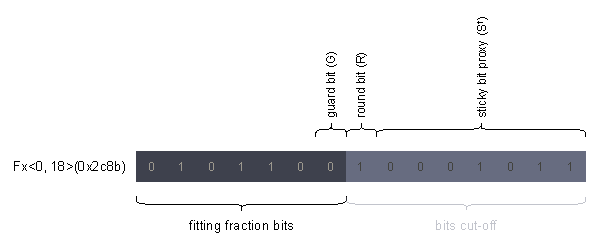
\includegraphics[width=\textwidth]{figures/bits-fraction.drawio.pdf}
    \caption{Bit-string layout of the fraction before rounding, with (G, R, S) bits highlighted}
    \label{fig:fraction_before_rounding}
    \end{center}
\end{figure}


\section{In-depth: division of fractions}\label{Approximated_Algorithms}
In this section, we will address the different existing solutions to compute the fractional part division.
% \footnote{explicit base 2 notation}
\begin{equation}
\frac{(1.f_1)}{(1.f_2)}
\end{equation}

When implemented in hardware, different non-negligible trade-offs come into play.

There are three main families of division algorithms \cite{muller_hardware_2010}. 

\begin{itemize}

\item Digit-recurrence (DR) algorithms, such as the family of SRT algorithms named after Sweeney, Robertson, and Tocher, %[344, 408]
generalize the paper-and-pencil algorithm. They produce one digit of the result at each iteration. Each iteration performs three tasks (just like the pencil-and-paper method): (i) determine the next quotient digit, (ii) multiply it by the divider, and (iii) subtract it from the current partial remainder to obtain a partial remainder for the next iteration.
In binary, there are only two choices of quotient digits, 0 or 1; therefore, the iteration reduces to one subtraction, one test, and one shift. 
A binary digit-recurrence algorithm can therefore be implemented on any processor as soon as it is able to perform integer addition.

One important thing about digit-recurrence algorithms is that they are exact. Starting from fixed-point numbers $X$ and $D$, they compute at iteration $i$ an $i$-digit quotient $Q_i$ and a remainder $R_i$ such that the identity $X = DQ_i + R_i$ holds.
For floating-point purposes, this means that all the information needed for rounding the result is held in the pair $(R_i, Q_i)$. In practice we limit the number of digits for the division result to $p$, introducing an approximation.
%In practice, to round to precision $p$, one needs $p$ iterations to compute $Q_p$, then possibly a final addition on $Q_p$ depending on a test on $R_p$.


\item Polynomial approximation can also be used to evaluate $1/x$ to the required accuracy. %[430].
Note that, mathematically speaking, functional iterations evaluate a polynomial in the initial approximation error. % [88].

\item Functional iteration algorithms generalize the Newton-Raphson iteration for approximating the function $1/x$. They make sense mostly on processors having a hardware multiplier. The number of iterations is much less than in digit-recurrence algorithms ($\mathcal{O}(\log p)$ versus $\mathcal{O}(p)$), but each iteration involves multiplications and is, therefore, more expensive. These latter two methods may be combined.
\end{itemize}

\subsection{Approximated reciprocal}

In order to compute an approximated reciprocate, we can think of exploiting the Taylor series technique\footnote{Wikipedia. 2022. "Taylor series." Wikimedia Foundation. Last modified October 4, 2022. https://en.wikipedia.org/wiki/Taylor\_series.} around $ 0.75 = mean([0.5, 1))$.


However, this approach presents some inconveniences:
\begin{itemize}
\item it requires $6$ fixed-point products\footnote{$3$ due to 3rd-order term $x*x*x*3.1604\dots$ + $2$ + $1$},
\item it is accurate just around the point where the series is expanded, as shown in figure \ref{fig:relative_error_00001}.
\end{itemize}
A way to circumvent the latter issue comes from employing the Chebyshev polynomials. They are used to provide the best approximation not only around a given point but across an interval.
As a trade-off, the better control over the accuracy across this interval comes at the cost of increased computational complexity, compared to the plain Taylor expansion.


Applying the third-order Chebyshev polynomials \cite{Hale2015}formula to $1/x$ across the interval $(0.5, 1)$ we obtain
\begin{equation}\label{equ:3rd_order_Chebyshev_polynomial_equation}
f_{cp_3} = 5.65685 - 11.75737x + 10.64818x^2 - 3.54939 x^3 + \mathcal{O}(x^4)
\end{equation}
which, from the visual comparison with other approximations (figure \ref{fig:relative_error_00001}) seems to return a better approximation of the $1/x$ function across the interval. However, similarly to the Taylor expansion, it still suffers from the long chain of fixed-point products.

A different idea comes from \cite{drom}, with a fast technique for approximated reciprocate computation. In particular, this approach offers three main advantages: (i) no dividers, except division by powers of $2$; (ii) minimal amount of multipliers; (iii) integer arithmetic only.


The following routine is indeed hardware friendly, as it employs just two integer multiplications and a bit shift.

\begin{verbatim}
def reciprocal(a):
    b = 1.466 - a
    c = a * b
    d = 1.0012 - c
    e = d * b
    out = e * 4
    return out
\end{verbatim}


\begin{figure}
    \centering
    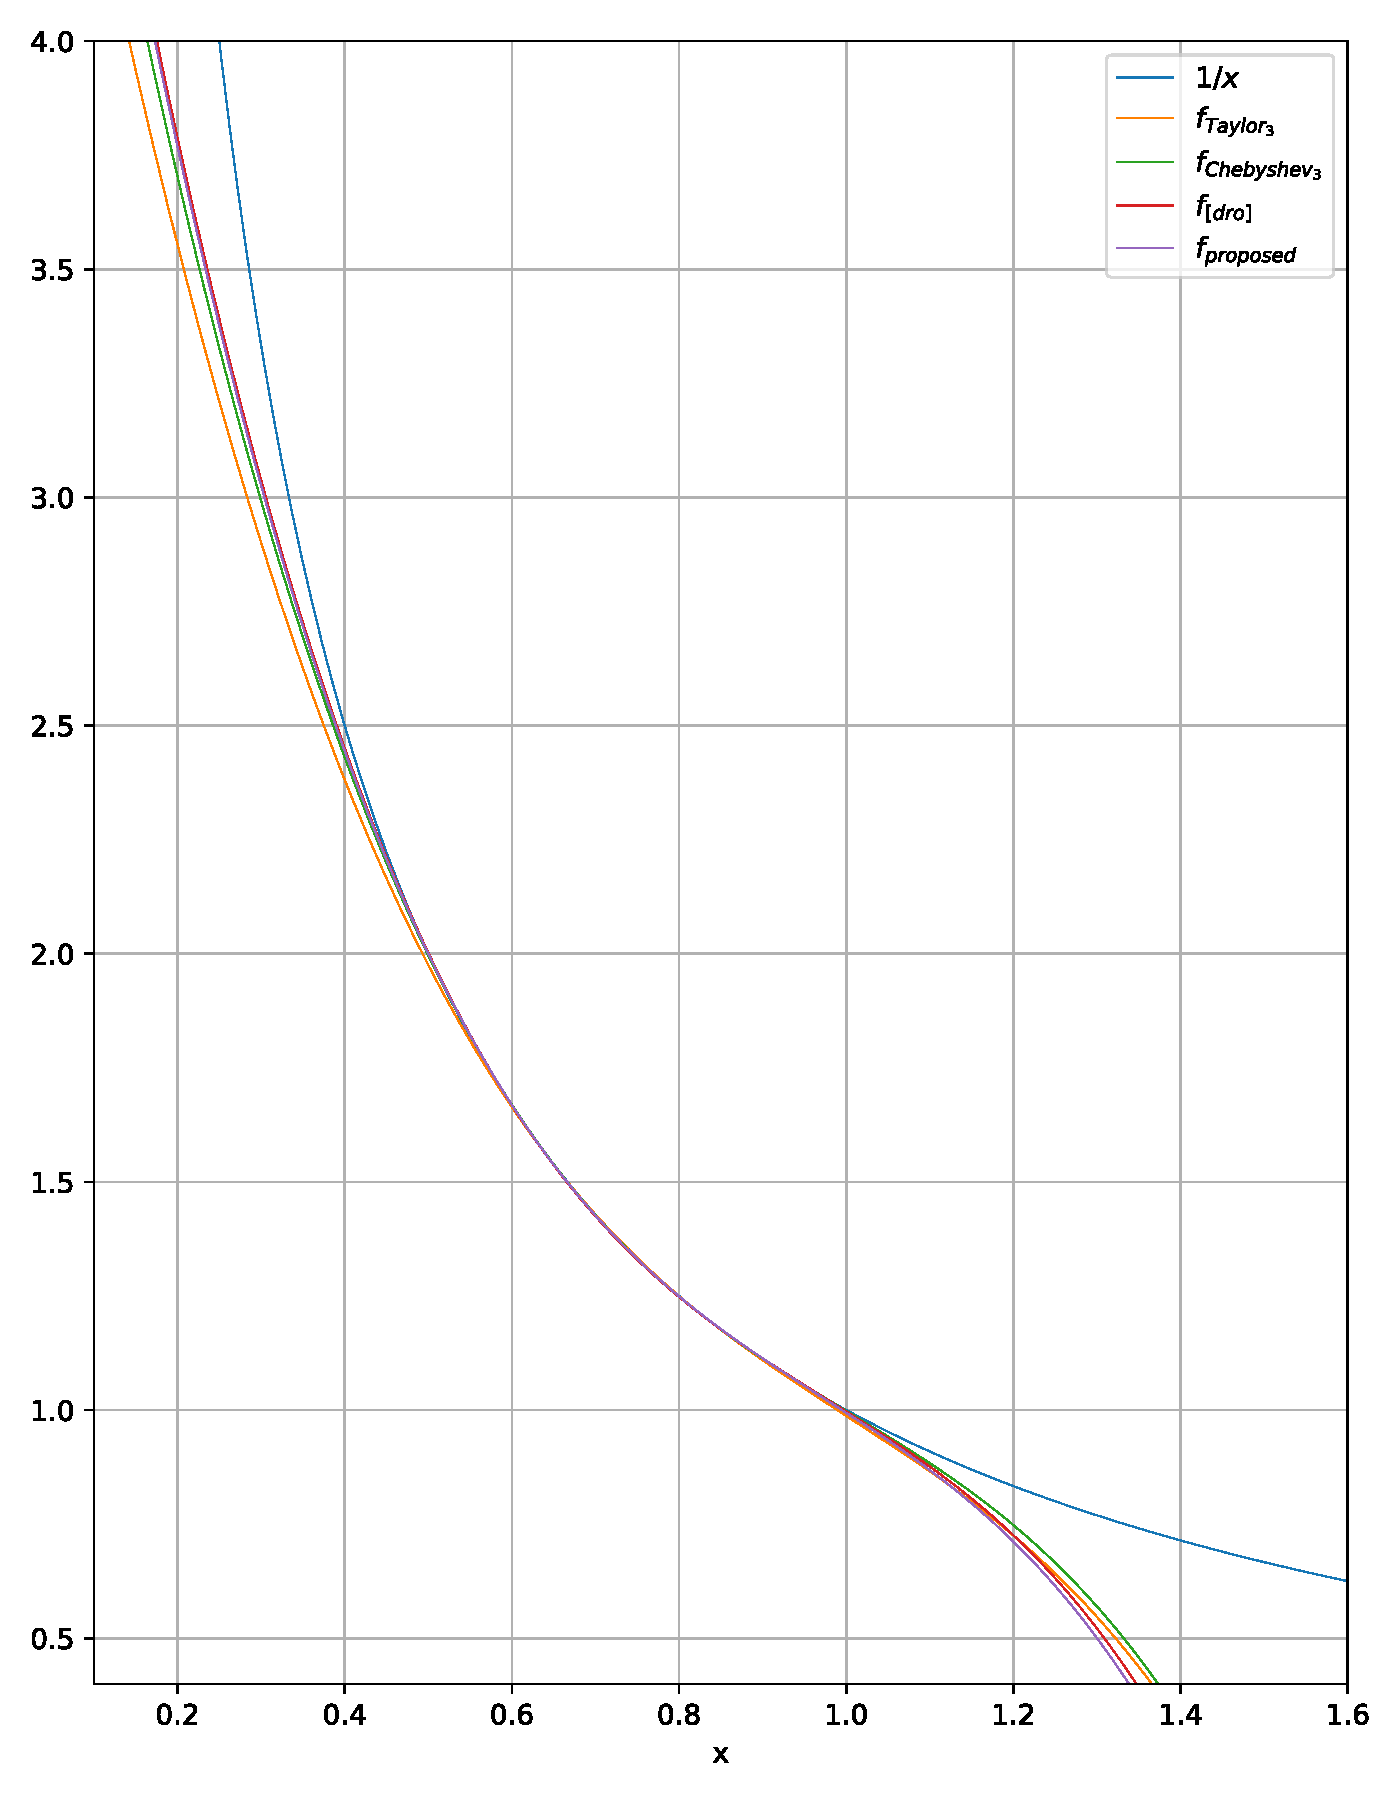
\includegraphics[width=0.75\textwidth]{figures/reciprocate_real_vs_taylor_vs_drom.pdf}
    \caption{Comparison of $1/x$ vs \cite{drom} vs 3rd order Taylor polynomial vs 3rd order Chebyshev polynomial vs proposed solution (i.e. optimized \cite{drom})}
    \label{fig:0203012875432985734}
\end{figure}

\begin{figure}
    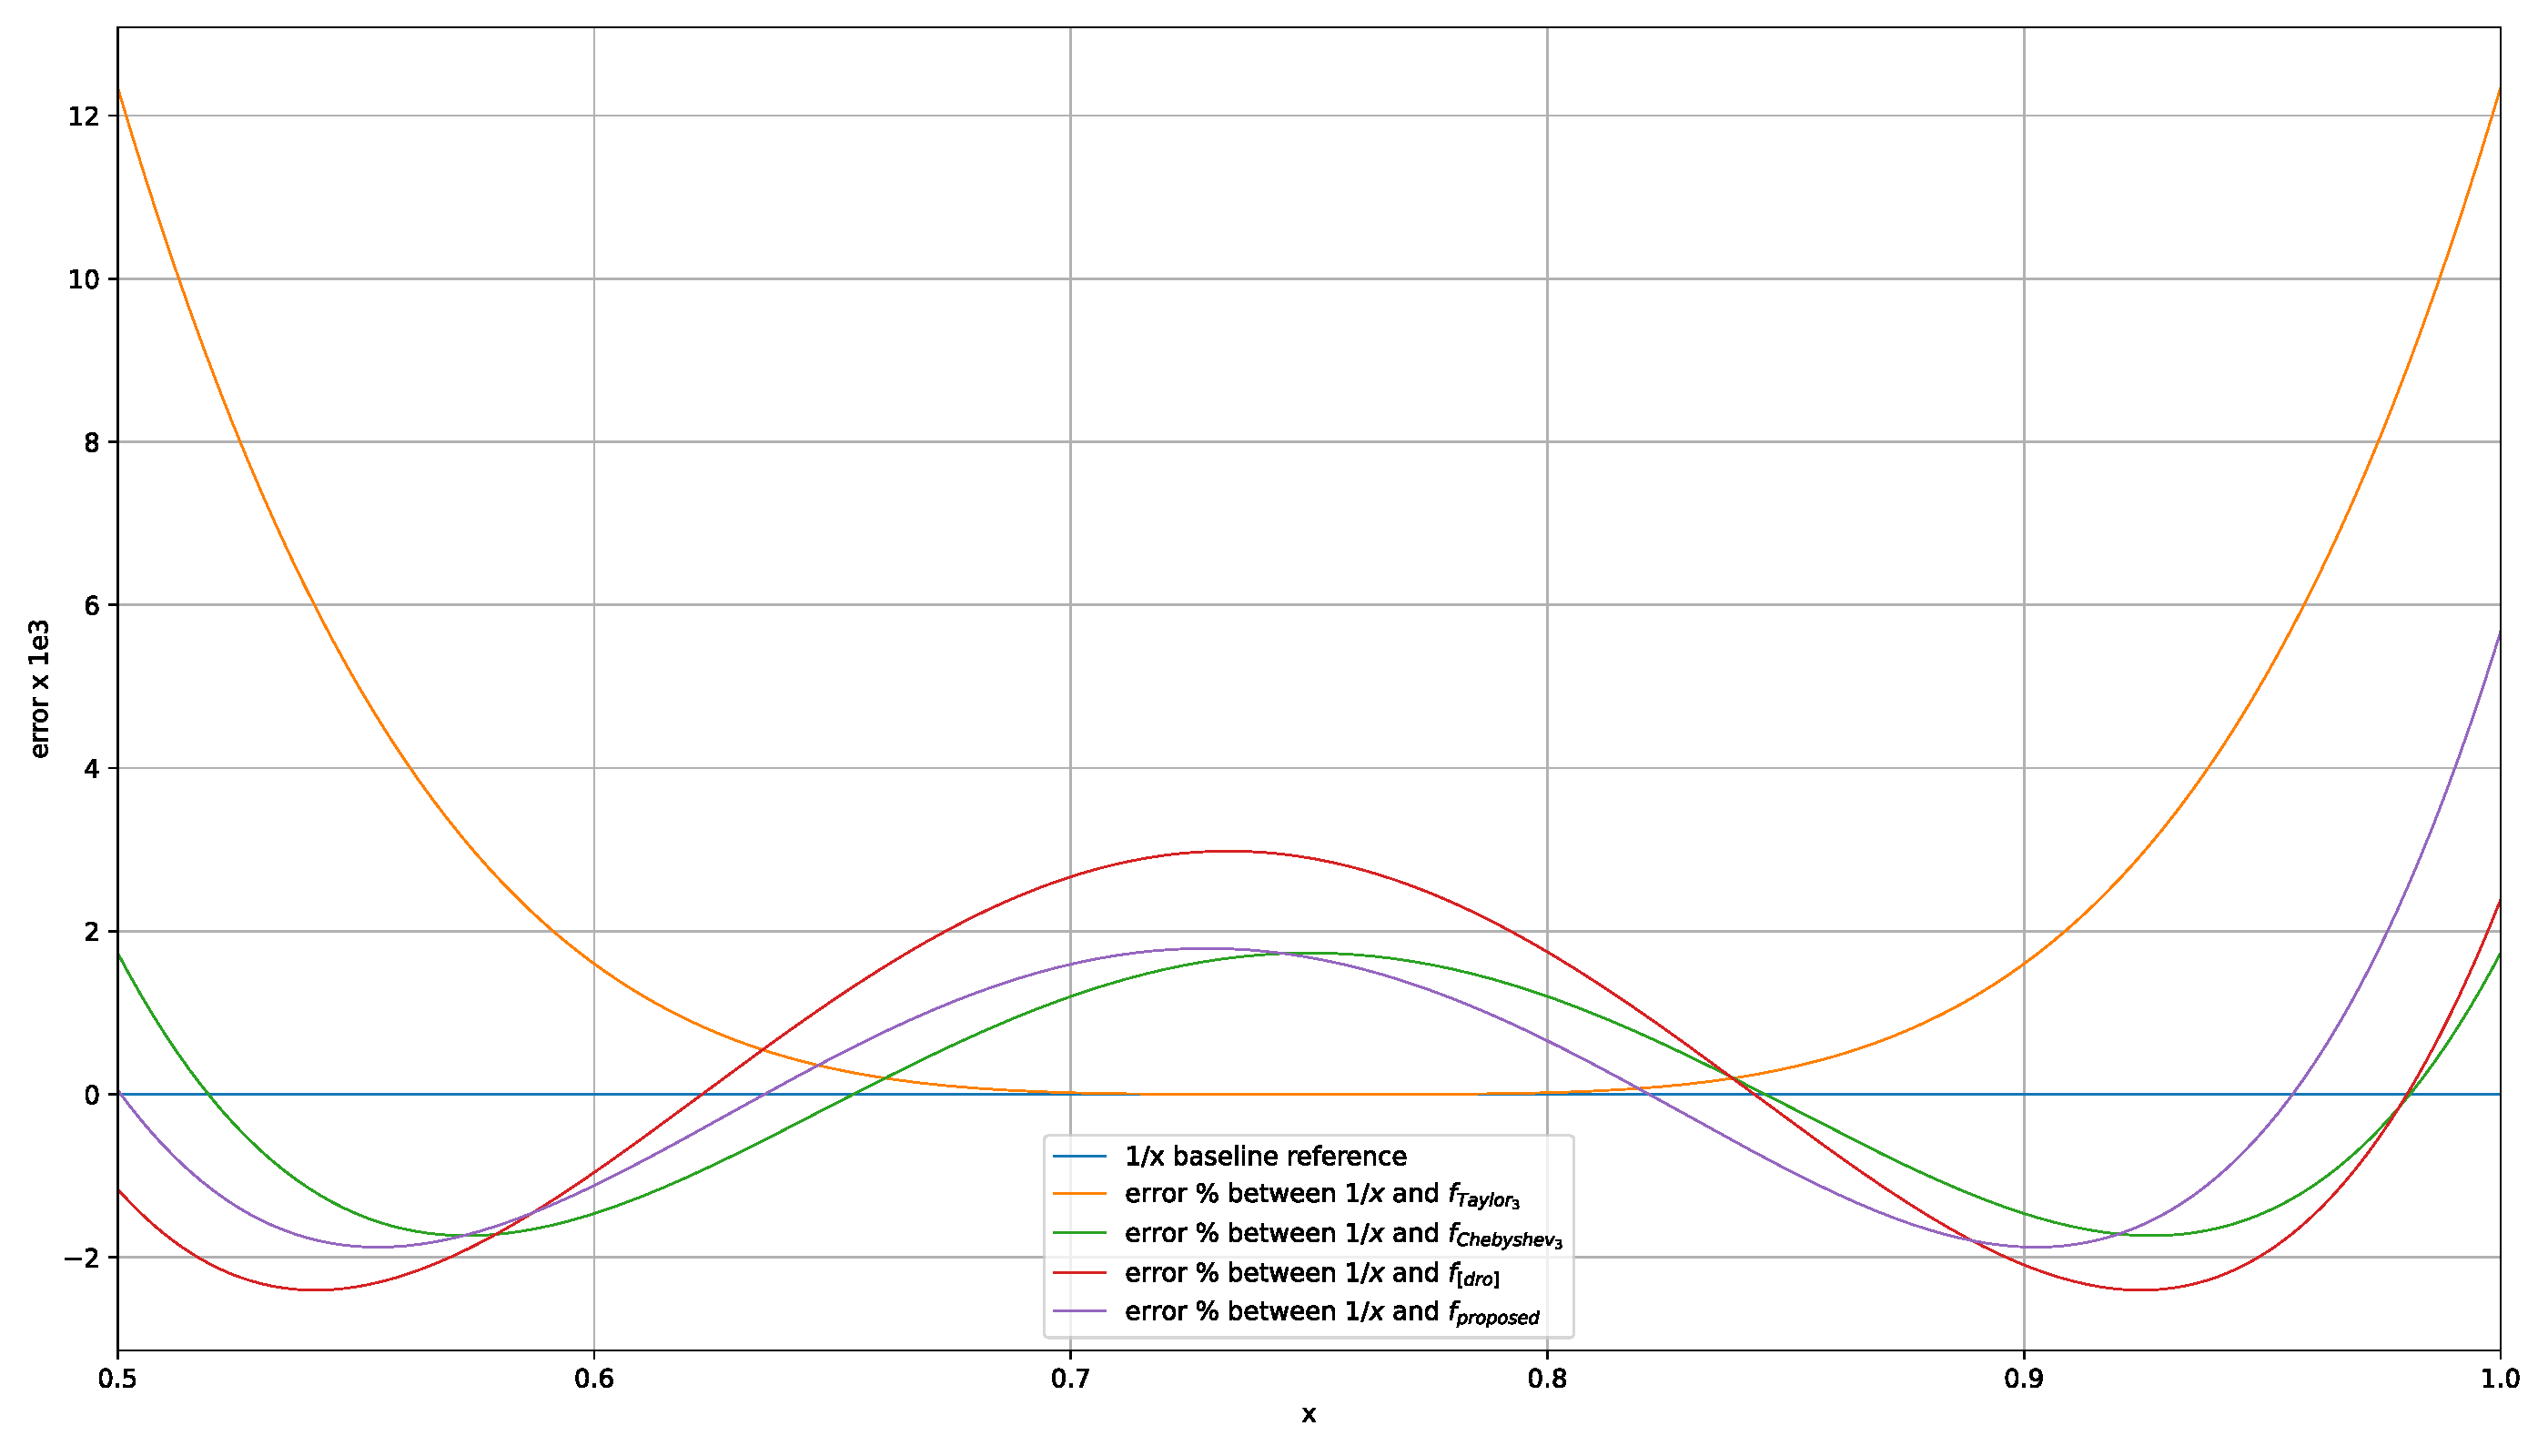
\includegraphics[width=1\textwidth]{figures/reciprocate_real_vs_taylor_vs_drom_error.pdf}\caption{Relative error against reference $1/x$}\label{fig:relative_error_00001}
\end{figure}
\begin{figure}
    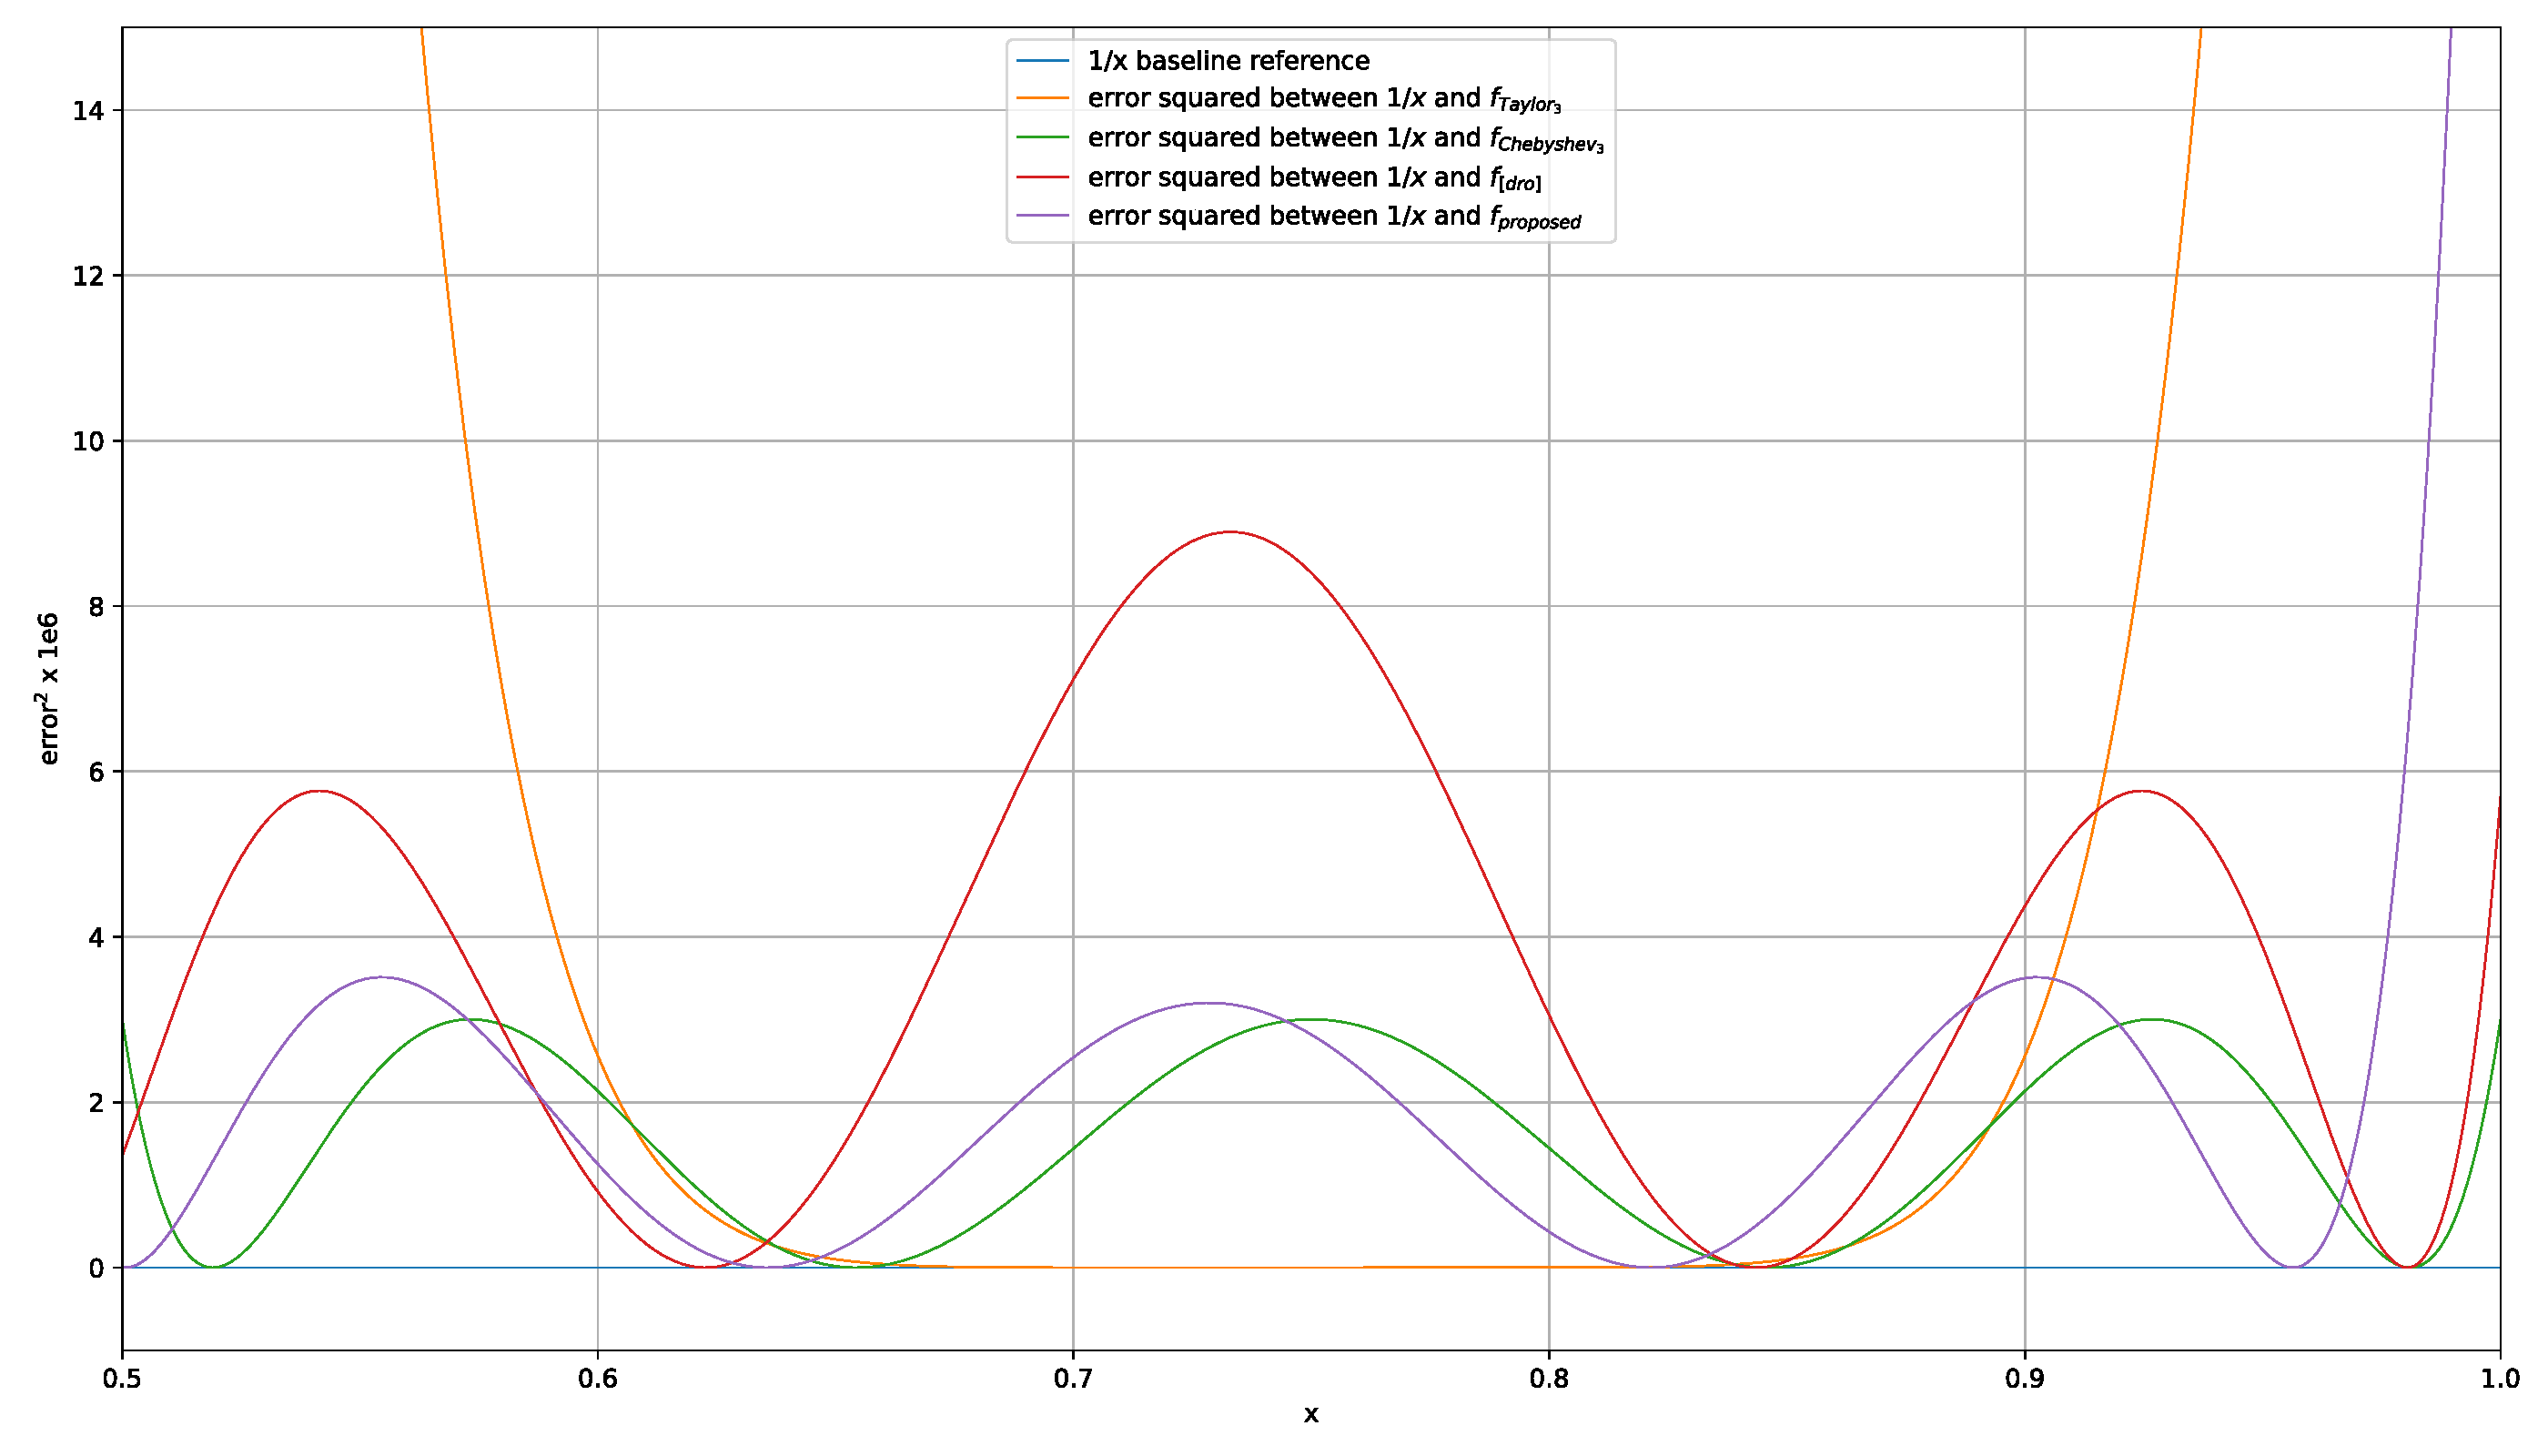
\includegraphics[width=1\textwidth]{figures/reciprocate_real_vs_taylor_vs_drom_error_squared.pdf} 
    \caption{Squared relative error against reference $1/x$}
    \label{fig:020301280980435232835} 
\end{figure} 

If we expand the routine into a  third-order polynomial (\ref{equ:expanded_drom_modified_polynomial}, \ref{equ:expanded_drom_0000}) similar to the previous ones, we can see that this is a modified Chebyshev polynomial with the highest grade coefficient rounded to the closest power of two -- $4$ in this case.
This constraint on the highest grade coefficient reduces the long-chained multiplication required by the original Chebyshev polynomial approximation (\ref{equ:3rd_order_Chebyshev_polynomial_equation}), with a slight degradation in accuracy.
\begin{equation}\label{equ:expanded_drom_modified_polynomial}
\begin{aligned}
f(a, k_1, k_2) &= 4 \cdot e = 4 \cdot d \cdot b = \\
&= 4 \cdot (k_2 - c) \cdot (k_1 - a) = \\
&= 4 \cdot (k_2 - a \cdot b) \cdot (k_1 - a) = \\
&= 4 \cdot [k_2 - a \cdot (k_1 - a)] \cdot (k_1 - a) = \\
&= 4 \cdot (k_2 - k_1 a + a^2) \cdot (k_1 - a) = \\
&= 4 \cdot (k_1 k_2 - k_2 a - k_1^2 a + 2 k_1 a^2 - a^3) = \\
&= 4 k_1 k_2 - 4(k_1^2 + k_2) a + 8 k_1 a^2 - 4 a^3
\end{aligned}
\end{equation}

Let $e^2$ be an error function to compare the accuracy of the different methods presented before. The function $e^2$ corresponds to the underlying area below the curves in Figure \ref{fig:020301280980435232835}. The value $rerr$ indicates the relative error between the real and the approximated function\footnote{$|rerr|$ would have given a comparably meaningful Function of Merit, however, the function must be differentiable in the entire domain, hence $rerr^2$}.


\begin{figure}
    \centering
    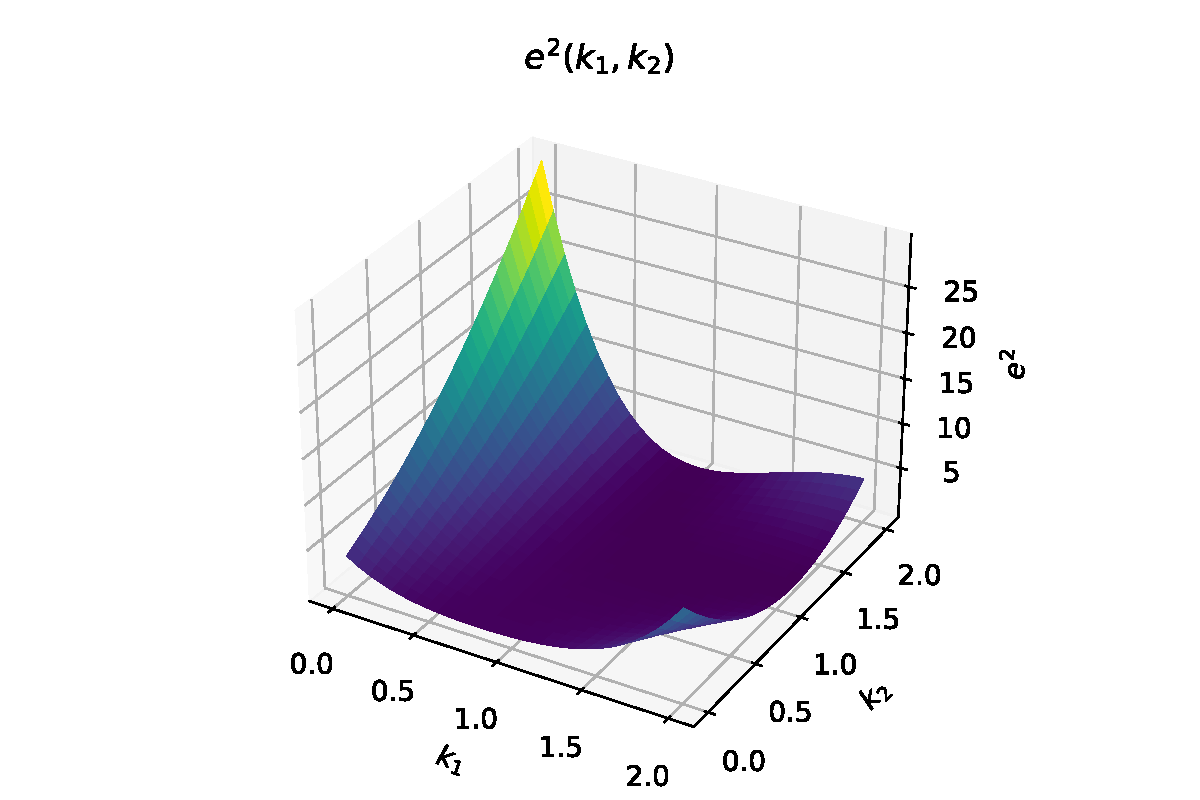
\includegraphics[
        %scale=1
        width=1\linewidth,]{figures/3d_plot_error_squared.pdf}
    \caption{\\$e^2(k_1, k_2)$}
    \label{fig:errorsquared3dplot}
\end{figure}
    
Let $f_{[dro]}$ be the Chebyshev polynomial defined using the coefficients as in \cite{drom}:

\begin{equation}\label{equ:expanded_drom_0000}
\begin{aligned}
f_{[dro]}(a) &= f(a, k_1=1.466, k_2=1.0012) = \\
&= 5.8710368 - 12.601424 a + 11.728 a^2 - 4 a^3
\end{aligned}
\end{equation}

 \begin{equation}\label{equ:equation_e_squared_k1k2}
            \begin{aligned}
            e^2(k_1, k_2) &=  \int_{1/2}^{1} rerr^2(x, k_1, k_2)\ dx = \\
            &= \int_{1/2}^{1} \left( \frac{f(x, k_1, k_2) - 1/x}{1/x} \right)^2 dx = \\
            &= \int_{1/2}^{1} \left( \frac{k_1 k_2 - 4(k_1^2 + k_2) x + 8 k_1 x^2 - 4 x^3 - 1/x}{1/x} \right)^2 dx = \\
            &= \frac{31 k_{1}^{4}}{10} - \frac{15 k_{1}^{3} k_{2}}{2} - \frac{21 k_{1}^{3}}{2} + \frac{14 k_{1}^{2} k_{2}^{2}}{3} + \frac{93 k_{1}^{2} k_{2}}{5} + \\ 
            &+ \frac{1339 k_{1}^{2}}{84} - \frac{15 k_{1} k_{2}^{2}}{2} - \frac{75 k_{1} k_{2}}{4} - \frac{375 k_{1}}{32} + \frac{31 k_{2}^{2}}{10} + \\ 
            &+ \frac{577 k_{2}}{84} + \frac{5507}{1440}
            \end{aligned}
        \end{equation}
        
We may want to know which are the optimal $k_1$ and $k_2$ such that:
\begin{equation}\label{equ:opt_k1_k2_eq}
(k_{1_{opt}}, k_{2_{opt}}): \min\{e^2(k_1, k_2)\}
\end{equation} 

For that the following system of equations (\ref{equ:opt_k1_k2_eq}) must be solved:
\begin{equation}\label{equ:opt_k1_k2_eq_partial}
\begin{cases}
\dfrac{\partial}{\partial k_1} e^2(k_1, k_2) = 0 \\
\dfrac{\partial}{\partial k_2} e^2(k_1, k_2) = 0
\end{cases}
\end{equation} 
\iffalse
$$
\begin{cases}
k_{1_{opt}} = 1.4567844114901045 \\
k_{2_{opt}} = 1.0009290026616422
\end{cases}
$$
\fi
which gives $(k_{1_{opt}} = 1.4567844114901045,\ k_{2_{opt}} = 1.0009290026616422)$, yielding a $36.4\%$ improvement over \cite{drom}'s $e^2$. Figure \ref{fig:are_barplot} shows a comparison of the relative accuracy of the above-mentioned functions and techniques compared to $1/x$.

\begin{figure}
    \begin{center}
    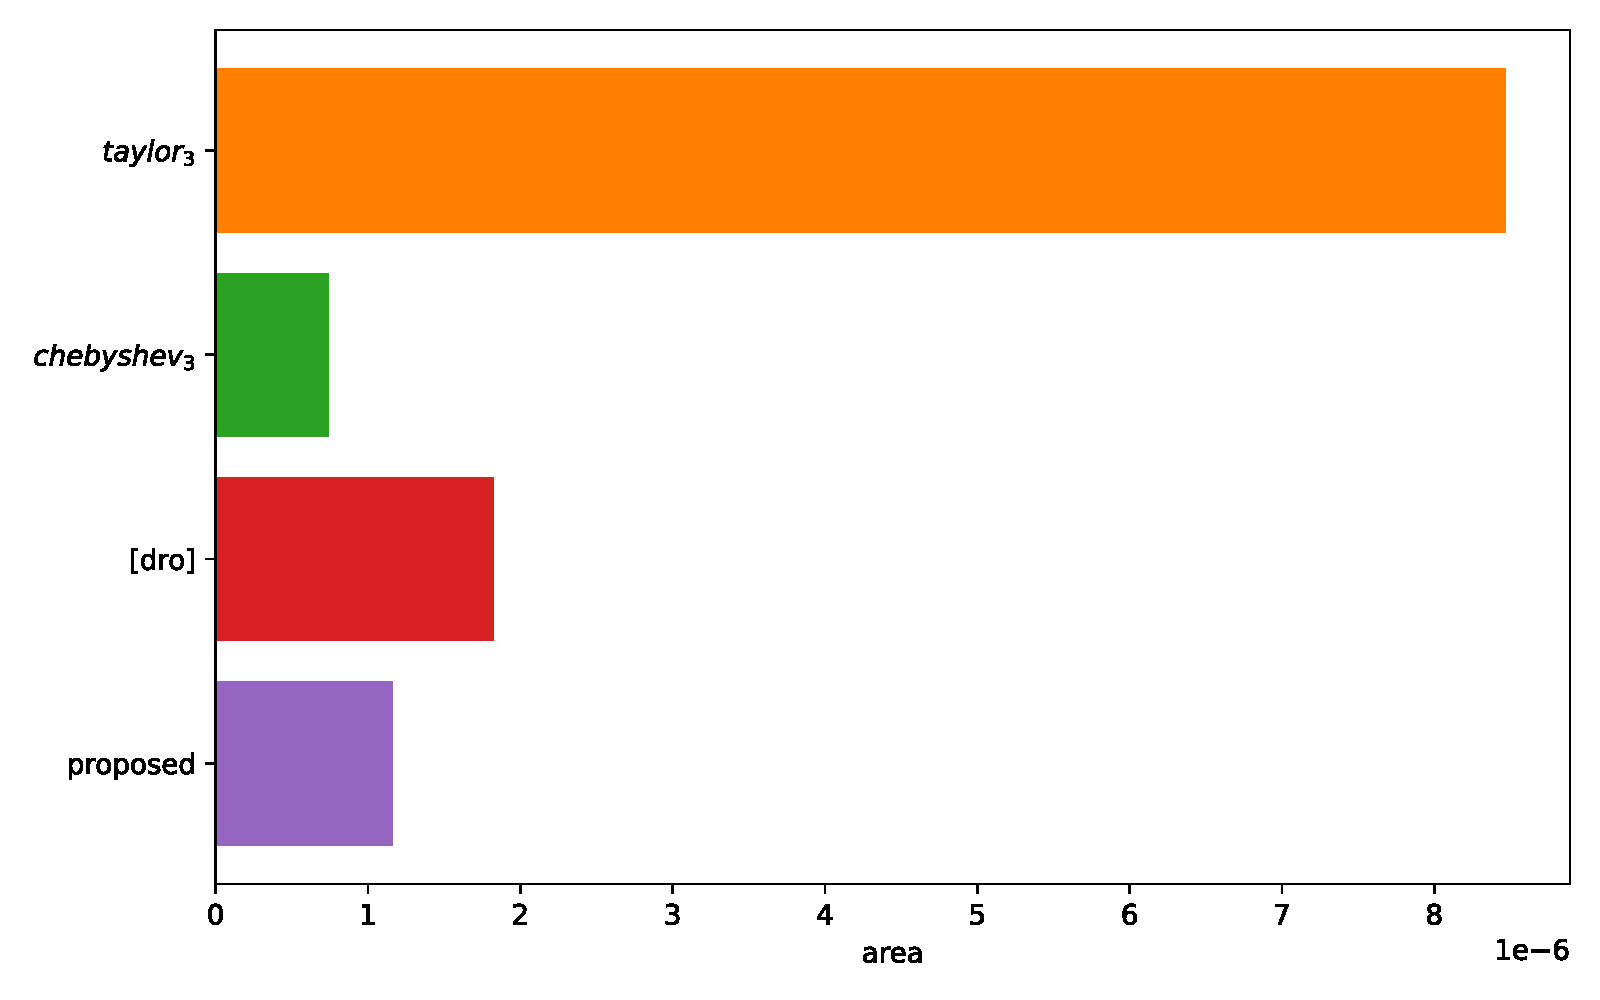
\includegraphics[width=0.4\textwidth]{figures/barplot_area_error.pdf}
    \caption{Barplot error area. $taylor_3$ vs $chebyshev_3$ vs \cite{drom} vs proposed}
    \label{fig:are_barplot}
    \end{center}
\end{figure}


Using the optimal $k_1$ and $k_2$ coefficients -- i.e. (i) Chebyshev-like polynomial, and (ii) highest grade coefficient being a power of $2$\footnote{so that the bit shift trick can be performed, as opposed to yet another multiplication} -- we can now use the following algorithm to perform the approximated reciprocal:

\begin{lstlisting}[label=alg:reciprocal_approx_modified_drom]
def reciprocal(a):
    b = k1_opt - a
    c = a * b
    d = k2_opt - c
    e = d * b
    out = e << 2
    return out
\end{lstlisting}

The numerical bounds of the result of each step in the algorithm can be determined so that we can set the correct fixed-point representation, allocating enough bits.

The input is a mantissa, hence contained in $[1, 2)$: in order to fit in the range required by the algorithm, that is $[0.5, 1)$, we divide by $2$, or, we just operate a one-bit right shift. Similarly, a division by $2$ is required when the algorithm terminates to restore the pre-normalization value.


Figure \ref{fig:reciprocal_unsigned_workflow} shows the flow of the procedure. 



\begin{itemize}
    \item \texttt{a} $\in [0.5, 1) \equiv A $ \dotfill \texttt{Fx<0, F>}
    \item \texttt{b} $\in (0.45702824, 0.95702824] $ \dotfill \texttt{Fx<0, F>}
    \item \texttt{c} $\in (0.45702824, 0.5307166278550605) $ \dotfill \texttt{Fx<0, 2F>}
    \item \texttt{d} $\in (0.47022002214493963, 0.54390841) $ \dotfill \texttt{Fx<0, 2F>}
    \item \texttt{e} $\in (0.24858150334349846, 0.4999731144222473) $ \dotfill \texttt{Fx<0, 3F>}
    \item \texttt{out} $\in (0.9943260133739938, 1.9998924576889892) $ \dotfill \texttt{Fx<1, 3F>}
\end{itemize}



    

\begin{figure}
    \centering
    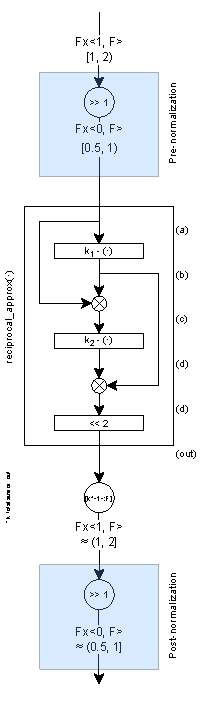
\includegraphics[width=0.28\textwidth]{figures/reciprocal_unsigned.drawio.pdf}
    \caption{Reciprocal unsigned workflow}
    \label{fig:reciprocal_unsigned_workflow}
\end{figure}

\subsection{Ahead-of-time reciprocal}\label{aot_reciprocal_lut_technique}

The previous solution presents a reduced result's precision (due to the approximated reciprocate) with the benefit of a reduction in required hardware resources.
Another solution called \textit{Ahead Of Time} computation of the reciprocate, helps with the accuracy drop seen before: the core idea is that instead of computing the reciprocate on-demand, we store the reciprocates inside a look-up table (as in \cite{PACoGen}). Such a look-up table takes $N$ bits representing the $N$ most significant bits of the fraction as input and will output the $M$ most significant bits of the reciprocate of the input.

\begin{figure}[h!]
    \begin{center}
    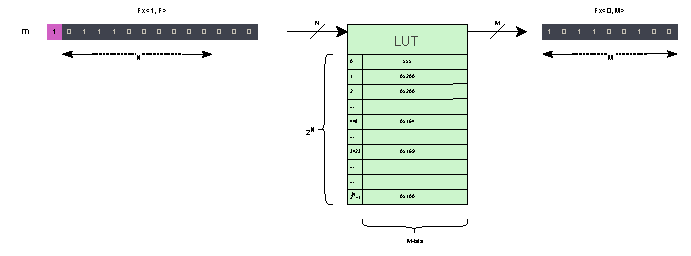
\includegraphics[width=1\textwidth]{figures/lut.drawio.pdf}
    \caption{Look Up Table example, taking P$\langle 16,1 \rangle(0x71c0)$'s mantissa as input}
    \label{fig:lut_drawio_example}
    \end{center}
\end{figure}

Concerning the same posit, $P\langle 16,1 \rangle(0x71c0)$, figure \ref{fig:lut_drawio_example} gives an example of the mechanism: i) the fraction field is adjusted to $N$ bits (this can be either a bit-expansion or a bit-compression); ii) the value represented by those bits is used to index the element in the look-up table resulting in the $M$ most significant bits of the reciprocate of the full input mantissa.

The lookup table gives another degree of freedom: $N$ and $M$ can be set independently from the posit size to account for the trade-off between resource utilization and required accuracy for the reciprocate.


\subsection{Newton-Raphson}\label{Newton_Raphson}


In numerical analysis, the Newton–Raphson method \cite{Hale2015_a} is a root-finding algorithm which produces successively better approximations of the roots of a real-valued function. The most basic version starts with a single-variable function $f$ defined for a real variable $x$, the function's derivative $f'$, and an initial guess $x_0$ for a root of $f$.
If the function satisfies sufficient assumptions and the initial guess is close, then the algorithm is guaranteed to converge to a root of $f$. The iterative scheme for the algorithm is shown in \eqref{equ:newon_raphson_generalized_equation}:

\begin{equation}\label{equ:newon_raphson_generalized_equation}
x_{n+1} = x_n - \frac{f(x_n)}{f'(x_n)}
\end{equation}

This technique can be exploited to solve the problem of interest by noticing that if we consider a function whose root is such that $x = 1/k$, e.g.
\begin{equation}
f(x) = \frac{1}{x} - k
\end{equation}
with derivative
$$
f'(x) = -\frac{1}{x^2}
$$
where $n$ is the number whose reciprocate we are after and $x$ the reciprocate itself, the Newton Raphson method gives
\begin{equation}
\begin{aligned}
x_{n+1} &= x_n - \frac{f(x_n)}{f'(x_n)} = \\
& = x_n - \frac{\dfrac{1}{x_n} - k}{-\dfrac{1}{x_n^2}} = \\
& = x_n\ (2 - k \cdot x_n)
\end{aligned}
\end{equation}
which yields a valid approximation so long as the initial guess $x_0 \in (0, 2/k)$, to not make the iteration diverge.


